\documentclass[output=paper]{langscibook}
\ChapterDOI{10.5281/zenodo.10280606}

\author{Catherine Felce\affiliation{Laboratoire Lidilem, Université Grenoble Alpes}}

\title[Linéarisation des énoncés en allemand langue débutée]{Linéarisation des énoncés en allemand langue débutée : Enseignement et développement dans une approche constructionniste}
      
\abstract{Dans cette contribution, je cherche à caractériser la manière dont les productions langagières de six apprenants grands débutants de l’allemand langue étrangère à l’université évoluent au cours du premier semestre d’apprentissage de la langue. Mon travail vise à mettre en relation les formes et expressions langagières que ces apprenants mobilisent dans des tâches de production avec les constructions sélectionnées et manipulées lors des activités en classe de langue. Je me place dans une perspective didactique qui interroge la nature des objets langagiers destinés à être enseignés en lien avec les enjeux acquisitionnels qui peuvent orienter leur sélection. En adoptant une conception de la langue et de la grammaire inspirée de l’usage et des grammaires de constructions, j'examine dans quelle mesure l’exposition à et la manipulation de constructions ciblées peuvent préparer l’émergence de structurations syntaxiques spécifiques de la langue cible chez des apprenants débutants. La proposition didactique formulée vise à familiariser les apprenants de manière précoce avec des options de linéarisation en L2 qui ne soient pas seulement correctes, mais conformes à l’usage en fonction du contexte discursif ou textuel des énoncés ; au-delà, il s’agit de poser des jalons susceptibles de dessiner un itinéraire d’apprentissage alternatif à la séquence développementale mise en évidence pour l’acquisition de l’ordre des mots en allemand.\smallskip\\
\textbf{Mots-clés:} langue débutée, didactique de l’allemand, approche basée sur l’usage, constructions, ordre des mots en allemand, trajectoires d’apprentissage}

\IfFileExists{../localcommands.tex}{
  \addbibresource{../localbibliography.bib}
  \usepackage{langsci-optional}
\usepackage{langsci-gb4e}
\usepackage{langsci-lgr}

\usepackage{listings}
\lstset{basicstyle=\ttfamily,tabsize=2,breaklines=true}

%added by author
% \usepackage{tipa}
\usepackage{multirow}
\graphicspath{{figures/}}
\usepackage{langsci-branding}

  
\newcommand{\sent}{\enumsentence}
\newcommand{\sents}{\eenumsentence}
\let\citeasnoun\citet

\renewcommand{\lsCoverTitleFont}[1]{\sffamily\addfontfeatures{Scale=MatchUppercase}\fontsize{44pt}{16mm}\selectfont #1}
   
  %% hyphenation points for line breaks
%% Normally, automatic hyphenation in LaTeX is very good
%% If a word is mis-hyphenated, add it to this file
%%
%% add information to TeX file before \begin{document} with:
%% %% hyphenation points for line breaks
%% Normally, automatic hyphenation in LaTeX is very good
%% If a word is mis-hyphenated, add it to this file
%%
%% add information to TeX file before \begin{document} with:
%% %% hyphenation points for line breaks
%% Normally, automatic hyphenation in LaTeX is very good
%% If a word is mis-hyphenated, add it to this file
%%
%% add information to TeX file before \begin{document} with:
%% \include{localhyphenation}
\hyphenation{
affri-ca-te
affri-ca-tes
an-no-tated
com-ple-ments
com-po-si-tio-na-li-ty
non-com-po-si-tio-na-li-ty
Gon-zá-lez
out-side
Ri-chárd
se-man-tics
STREU-SLE
Tie-de-mann
}
\hyphenation{
affri-ca-te
affri-ca-tes
an-no-tated
com-ple-ments
com-po-si-tio-na-li-ty
non-com-po-si-tio-na-li-ty
Gon-zá-lez
out-side
Ri-chárd
se-man-tics
STREU-SLE
Tie-de-mann
}
\hyphenation{
affri-ca-te
affri-ca-tes
an-no-tated
com-ple-ments
com-po-si-tio-na-li-ty
non-com-po-si-tio-na-li-ty
Gon-zá-lez
out-side
Ri-chárd
se-man-tics
STREU-SLE
Tie-de-mann
} 
  \togglepaper[1]%%chapternumber
}{}

\begin{document}
\begin{otherlanguage}{french}
\AffiliationsWithoutIndexing{}
\lsFrenchChapterSettings{}
\maketitle 
% Keywords: beginner learners, usage-based approach, constructions, German as a Foreign Language (GFL), German word order, developmental trajectories

\section{Introduction}\label{sec:felce:1}

Débuter l’apprentissage d’une nouvelle langue à l’âge adulte peut recouvrir une variété de situations, de conditions d’apprentissage et de degrés de réussite. Que les apprenants soient des travailleurs migrants, des individus contraints, pour des raisons diverses, de quitter leur pays d’origine ou encore des étudiants choisissant une langue nouvelle pour eux comme option dans leur cursus universitaire, les progrès de ces apprenants dans leur appropriation de la langue cible (désormais LC) dépendront de multiples facteurs (\citealt{Dörnyei2009psychology, DörnyeiRyan2015}). Ces derniers peuvent être liés à des dispositions ou des aptitudes individuelles, à des connaissances langagières relatives à d’autres langues acquises et disponibles, ou aux conditions externes qui caractérisent les situations d’usage et d’apprentissage de la LC ; au-delà de ces différences individuelles, des points communs ont pu être mis en évidence dans le cadre de différents programmes de recherche menés au tournant des années 1970–1980,\footnote{On pense notamment aux programmes ESF (\textit{European Science Fondation}) et ZISA (\textit{Zweit\-sprach\-er\-werb italienischer und spanischer Arbeiter}). On peut se reporter à \citet[43--51]{Véronique2009} pour une description synthétique des différents programmes de recherche menés dans une perspective longitudinale.} puis dans des travaux ultérieurs qui ont contribué à la compréhension et à la description d’une dynamique de l’appropriation à partir de corpus d’apprenants (\citealt{BartningSchlyter2004, Myles2008}).

Si la recherche en acquisition des langues (désormais RAL) s’est tournée à l’époque de son établissement comme discipline scientifique de manière privilégiée vers des contextes d’acquisition dits naturels –  s’éloignant un temps de préoccupations liées à l’enseignement et, ce faisant, de la didactique des langues \citep{Véronique2005Interrelations} – les appels et les travaux visant à promouvoir le dialogue entre recherches acquisitionnistes et enjeux didactiques sont revenus depuis un peu plus d’une décennie sur le devant de la scène dans le domaine francophone (\citealt{Komur-ThilloyTrévisiol-Okamura2011, Véronique2017, WatorekEtAl2021eds}). 

La présente contribution relève de cette même ambition visant à s’appuyer sur la compréhension de processus d’apprentissage pour orienter les démarches instructionnelles. Notre réflexion part des activités d’enseignement mises en œuvre sur le terrain pour les interroger à la lumière d’approches linguistiques et de travaux qui se sont intéressés à l’ordre des mots et à la structuration de l’énoncé en allemand en lien avec les possibilités de leur enseignement (\citealt{Pienemann1999, DiehlEtAl2000, Winkler2017}). Notre intérêt se porte plus particulièrement sur l’apprentissage de l’allemand au niveau débutant, dans le contexte universitaire qui est celui d’étudiants spécialistes d’autres disciplines démarrant l’apprentissage de cette langue comme option dans leur cursus. Pour ces apprenants, l’option de langue constitue souvent une L3 voire une L4,\footnote{Je ne ferai pas de distinction et parlerai de L2 pour désigner toute langue apprise postérieurement à l’acquisition de L1, indépendamment de l’ordre d’acquisition de ces langues additionnelles.} débutée à l’âge adulte dans un contexte guidé et hétéroglotte. C’est en référence à ce public particulier et à ce contexte d’apprentissage que je parle de «~langue débutée~».

Notre contribution traite de la manière d’accompagner ces apprenants vers la réalisation d’options de linéarisation s’éloignant d’un ordre des mots de type Sujet-Verbe, de manière à en soutenir, voire à en favoriser l’appropriation. Quelle approche de la langue (et de la grammaire) privilégier pour cela avec des groupes d’apprenants très hétérogènes (de par la diversité de leurs L1, de leurs cultures éducatives et de leurs motivations)~et peu familiers d’une terminologie grammaticale ? Comment, dès les débuts de l’apprentissage, préparer le terrain~en familiarisant les apprenants avec des choix de linéarisation adéquats en fonction du contexte situationnel ou textuel donné et en les amenant à privilégier l’usage de ces options dans leurs productions ? Par quel biais favoriser l’acquisition précoce d’expressions langagières qui puissent, ultérieurement, donner lieu à la reconnaissance de patrons ouverts à des recompositions (lexicales ou morphologiques) en fonction du contexte et évoluant vers une productivité plus grande ? À l’opposé d’une vision formelle de la grammaire conçue comme un ensemble de règles appliquées aux mots, j'adopte dans cette étude une perspective qui considère que l’évolution du système langagier met en jeu des schémas reconnus dans différentes expressions par le biais de mécanismes cognitifs généraux (analogie, catégorisation, généralisation, \citealt{Diessel2007}) et qui postule un continuum entre lexique et grammaire (\citealt[90–95]{ZiemLasch2013}).

J'aborde dans une première partie la question de la construction de l’énoncé à travers la description linguistique qui la caractérise, puis à travers la dynamique développementale propre à l’ordre des mots mise en évidence dans le cadre du projet ZISA (\citealt{MeiselEtAl1981, ClahsenEtAl1983}).

\begin{sloppypar}
La deuxième partie de cette contribution me permettra de mettre en regard des travaux de deux types portant sur l’enseignement-apprentissage d’une langue seconde en contexte guidé. Les uns visant à en étudier les mécanismes ou les trajectoires d’appropriation à partir de cadres théoriques de la recherche en acquisition, les autres, motivés par des préoccupations de terrain et interrogeant la pertinence de l’intervention pédagogique sur la base de résultats ou de notions issus de travaux du domaine. Cette mise en perspective me servira à expliciter mon positionnement entre les champs de la didactique des langues et de la RAL. 
\end{sloppypar}

Ces deux premières parties me conduiront à formuler de nouvelles propositions pour aborder la grammaire au niveau débutant ; des développements à partir d’une approche cognitive et constructionniste de la grammaire feront alors l’objet d’une troisième partie.

Ces jalons théoriques une fois posés, j'étudierai l’évolution des choix langagiers observables dans les performances de six apprenants débutant l’apprentissage de l’allemand à l’université. À cette fin, cinq de leurs productions langagières recueillies au début et à la fin du premier semestre d’apprentissage seront analysées. Les analyses, mises en relation avec les moyens langagiers travaillés en classe de langue, s’orienteront en fonction des questions de recherche suivantes : 

\begin{enumerate}\sloppy
\item[Q1.] Quelles constructions les apprenants mobilisent-ils de manière privilégiée dans leurs productions langagières ?

\item[Q2.] Peut-on mettre en évidence une évolution dans la manière dont ces expressions sont mobilisées dans les productions~et que retenir de cette évolution ?

\item[Q3.] Est-il enfin possible de reconnaitre à certains patrons ou à certaines associations mémorisées un potentiel de productivité de telle sorte qu’ils puissent être considérés comme des paliers vers des réalisations syntaxiques conformes à la LC ?
\end{enumerate}

\begin{sloppypar}
Ces analyses ont à ce stade un caractère exploratoire ; elles doivent permettre, d’une part, de poser les bases d’une possible méthodologie destinée à étudier l’évolution du système langagier d’apprenants débutants dans une approche constructionniste du développement et, d’autre part, d'orienter ou réorienter les activités d’enseignement afin de faciliter l’entrée dans la langue chez ces apprenants. 
\end{sloppypar}

Mon propos sera par ailleurs irrigué par des réflexions inspirées de celles que Daniel Véronique a mises en avant dans plusieurs de ses articles qui articulent réflexion didactique et recherches acquisitionnistes.

\section{Construction de l’énoncé en allemand et ordre des mots}\label{sec:felce:2}
\subsection{Une double description linguistique}\label{sec:felce:2.1}

Les descriptions formelles de l’allemand mettent en avant des spécificités liées à la linéarisation des constituants de l’énoncé. L’une de ces spécificités réside dans la manière d’appréhender la structure du groupe verbal à l’infinitif (OVinf). Si, en français, les constituants s’organisent partant du verbe dans une logique de progressivité, on parle en allemand d’ordre régressif dans la mesure où la position finale du verbe non fléchi admet des expansions qui se font de la droite vers la gauche : dans la structure syntagmatique de l’allemand, les connexions sémantiques s’établissent «~à rebours~» de la linéarisation de surface. 


\begin{figure}
\begin{tikzpicture}
	\node at (0,0) [single arrow, draw, shape border rotate=180] 
	  {\begin{tabular}{@{} c @{}}
	  	\multicolumn{1}{r}{\itshape Deutsch       \textbf{lernen}}\\
	  	\multicolumn{1}{r}{\itshape Deutsch lernen \textbf{wollen}}\\
	  	\multicolumn{1}{l}{`\textbf{apprendre} l’allemand'} \\
	  	\multicolumn{1}{l}{`\textbf{vouloir} apprendre l’allemand'} \\
	  \end{tabular}};
\end{tikzpicture}
\caption{Structure du groupe verbal en allemand\label{fig:felce:1}}
\end{figure}

\begin{sloppypar}
Une autre spécificité reconnue à l’allemand concerne la linéarisation de surface. Pour en rendre compte, on a communément adopté un découpage en «~champs~», (\textit{Vorfeld – Mittelfeld – Nachfeld}) (\tabref{tab:felce:1}), dans lesquels les différents constituants de l’énoncé se répartissent selon une structure topologique \citep{Wöllstein2014}.
\end{sloppypar}

\begin{table}
\tabcolsep=.66\tabcolsep\small%
\begin{tabular}{l@{~}ccccc}
\lsptoprule
     & Champ initial &  & Champ médian &  & Champ terminal\\
     & \textit{(Vorfeld)} &  & \textit{(Mittelfeld)} &   & \textit{(Nachfeld)}\\\midrule
% Position préverbale & \multicolumn{3}{c}{sentence bracket \quad \quad \textit{Satzkklammer}} & \\\midrule
     & X & Vfin (V2) & & Vinf & \textbf{Vinf + Vfin}\\\midrule
(1)  & \textit{ich} & \textit{lerne} & \textit{Deutsch} & & \\\relax
     & {`je/j'} & apprends & {l'allemand'} & & \\\addlinespace\addlinespace
(2)  & \textit{ich} & \textit{will} & \textit{Deutsch} & \textit{lernen} & \textit{, weil ich in Deutschland}\\\relax
     &  & & & & \textit{\textbf{arbeiten möchte}}\\
     &  {`je/j'} & veux & l`allemand & apprendre & , parce que je voudrais \\
     &  & & & & {travailler en Allemagne'} \\\addlinespace\addlinespace
(3)  & \textit{dieses Jahr} & \textit{will} & \textit{ich Deutsch} & \textit{lernen} & \\\relax
     & `cette année & veux & je l`allemand & apprendre & \\
\lspbottomrule
\end{tabular}
\caption{Modèle topologique de l’énoncé assertif et positionnement des formes verbales\label{tab:felce:1}}
\end{table}

Au sein même de cette répartition, deux caractéristiques méritent d’être soulignées. La première concerne la contrainte positionnelle associée aux éléments verbaux finis et non finis, placés respectivement en deuxième (Vfin ou V2) et en dernière position (Vinf)\footnote{Ou encore (Vinf) + Vfin dans les subordonnées telles que celle donnée en exemple (\tabref{tab:felce:1}).} et qui forment une parenthèse verbale (\textit{sentence bracket}) enserrant les constituants positionnés dans le champ médian. La seconde caractéristique réside dans l’hétérogénéité des éléments positionnés dans le champ initial, c’est-à-dire en position préverbale, et à la variabilité associée à l’occupation de ce champ. En effet, le \textit{Vorfeld} n’est pas une position syntaxiquement déterminée (\citealt[1584]{ZifonunEtAl1997}) ; elle n’est pas réservée au sujet comme c’est généralement le cas en français ou en anglais~mais peut être occupée par des constituants de nature et de structure très diverses. En allemand, il est ainsi fréquent de voir apparaître le sujet après le verbe fléchi, la première position étant alors occupée par un autre constituant (des adverbiaux ou groupes prépositionnels cadratifs, des éléments relevant du thème, des attaques rhématiques, des appréciatifs, entre autres).

D’un point de vue acquisitionnel, des travaux de référence ont montré que le positionnement correct des formes verbales fait partie des points qui résistent à l’instruction (\citealt{Ellis1989}, \citealt{Pienemann1989}) dans le cas de langues sources de type SVO~et établi que l’acquisition de l’ordre des mots en allemand L2 suit une trajectoire acquisitionnelle bien spécifique.

\subsection{Séquence développementale relative à l’ordre des mots} \label{sec:felce:2.2}

Les programmes de recherche évoqués plus haut ont étudié l’acquisition de différentes langues secondes dans le but de retracer les itinéraires d’apprentissage de travailleurs étrangers, souvent peu scolarisés, venus en Europe en réponse aux besoins de main d’œuvre et confrontés à la langue de leur nouvel environnement en dehors de tout guidage instructionnel.\footnote{Daniel Véronique a été de l’équipe (aux côtés entre autres de Wolfgang Klein et Clive Perdue) qui, dans le cadre du projet \textit{The ecology of adult language acquisition} (EALA) dit aussi ESF (\textit{European Science Found\-a\-tion}), du nom de la fondation qui l'a soutenu, a contribué à décrire les trajectoires d’appropriation de ces apprenants et à caractériser leur progrès dans la langue apprise en termes de variétés langagières \citep{Perdue1993vol2}} En amont du projet EALA, les programmes \textit{Heidelberger Forschungsprojekt} \textit{«~Pidgin\-deutsch~»} (HPD) (\citealt{DittmarKlein1975}) et ZISA (\textit{Zweitspracherwerb italienischer und spanischer Arbeiter}) (\citealt{MeiselEtAl1981}) ont étudié la manière dont des travailleurs originaires du bassin méditerranéen progressaient dans l’acquisition des propriétés syntaxiques de l’allemand. Le programme ZISA est souvent cité en référence à la séquence relative à l’acquisition de l’ordre des mots en allemand. 

\begin{table}
\fittable{\begin{tabular}{l@{~~}ll}
\lsptoprule
(1, 2)  & Stade $x$ & \textit{\textbf{die kinder spielen mim ball}}\\
        & (Canonical Order) & `the children play with the ball'\\
(3)     & Stade $x + 1$  & \textit{\textbf{da} kinder spielen}\\
        & (Adverb Preposing) (XSVfin) & `there children play'\\
(4)     & Stade $x + 2$  & \textit{alle kinder \textbf{muss} die pause \textbf{machen}}\\
        & (Verb Separation) (Vfin-OVinf)                                 & `all children must the break have'\\
(5)     & Stade $x + 3$   & \textit{\textbf{dann hat} sie wieder die knoch gebringt}\\
        & (Inversion) (XVfinS) &  `then has she again the bone bringed'\\
(6)     & Stade $x + 4$  & \textit{er sagt, dass er nach hause \textbf{kommt}}\\
        & (Verb Final) (SOVfin) & `he says that he home comes'\\
\lspbottomrule
\end{tabular}}
\caption{Hiérarchie des stades d’acquisition (ZISA) (\citealt[45]{Pienemann1999}). Les exemples sont ceux de Pienemann.\label{tab:felce:2}}
\end{table}
 

En mettant en évidence une hiérarchie dans l’ordre d’acquisition des structures (\tabref{tab:felce:2}), les chercheurs ont établi que la progression des locuteurs dans leur appropriation de l’ordre des mots était soumise au développement graduel de stratégies cognitives rendant possible le traitement d’une structure donnée à différents stades identifiés, chaque palier constituant un prérequis pour l’accession au palier supérieur. Ces travaux, initialement menés en contexte non guidé, ont conduit à des interrogations sur l’enseignabilité (\textit{teachability}) des structures de la L2 et sur les limites de l’intervention enseignante (\citealt{Pienemann1984, Pienemann1989, Ellis1989}). Si la disponibilité des procédures de traitement contraint la progression, alors l’apprentissage d’une structure relevant d’un stade pour lequel un apprenant ne serait pas encore prêt ne peut pas être forcé.

\begin{quote}
\begin{otherlanguage}{english}
“Skipping stages” in formal instruction would imply that there would be a gap in the processing procedures needed for the learner’s language. Since all processing procedures underlying a structure are required for the processing of the structure, the learner would simply be unable to produce the structure.\hbox{}\hfill\hbox{\citep[13]{Pienemann1999}}
\end{otherlanguage}
\end{quote}

Les travaux initiés dans le cadre du projet ZISA ont par la suite conduit Pienemann à élaborer une théorie explicative pour la dynamique de l’appropriation~(\textit{Processability Theory}) et différentes études menées en référence à cette théorie ont contribué à l’élaboration d’un modèle théorique qui a certes évolué vers la reconnaissance de possibles variations dans les parcours identifiés, mais qui n’en demeure pas moins un modèle éprouvé (\citealt{Håkansson2005, Pienemann2005, PienemannKeßler2011}). Plusieurs travaux ultérieurs menés en contexte guidé ont confirmé la robustesse de la séquence développementale relative à l’ordre des mots en allemand L2 (\citealt{Boss2004, Jansen2008, Ballestracci2010}) et contribué à soutenir les arguments formulés en faveur d’une prise en compte de ces résultats dans les curricula \citep{DiehlEtAl2000}.

Notre propos n’est pas de remettre en cause les stades de développement tels qu’ils ont été élaborés dans leur cadre de référence, mais de réinterroger cette séquence acquisitionnelle à la lumière d’une approche constructionniste du développement langagier, observé notamment en début d’apprentissage.

\section{L’enseignement-apprentissage d’une «langue débutée»}\label{sec:felce:3}
\begin{sloppypar}
J'ai fait le choix de parler de «langue débutée» pour caractériser les langues apprises dans un contexte guidé et hétéroglotte à l’âge adulte, c’est-à-dire postérieurement l’acquisition de la L1 (ou langue de première socialisation) et parfois même après l’apprentissage d’une, voire de plusieurs L2. Dans ce contexte (LANSAD\footnote{LANgues pour Spécialistes d’Autres Disciplines.}), le choix d’apprendre une langue additionnelle se fait dans le cadre du cursus universitaire des apprenants,~qui peuvent non seulement avoir des affiliations disciplinaires très variées, mais aussi des origines culturelles diverses.\footnote{Se reporter au \tabref{tab:felce:3} en \sectref{sec:felce:5.1} pour une description de l’échantillon dont il est question dans cette étude.} Par rapport au choix de la langue, ces derniers mentionnent souvent la curiosité et l’envie de découverte ou ont parfois des objectifs instrumentaux à plus long terme ; on retient surtout que les motivations et les ambitions affichées peuvent s’avérer très disparates, rendant les parcours d’apprentissage discontinus et l’investissement dans l’apprentissage inégal.
\end{sloppypar}

Concernant les débuts de l’apprentissage de L2 en contexte guidé et le lien avec l’enseignement, les travaux peuvent se distinguer dans leur intention initiale : certains travaux se situant dans le champ de la RAL visent à décrire et étudier les processus acquisitionnels dans différentes configurations d’enseignement, alors que d’autres travaux, initiés par des praticiens, relèvent d’une orientation didactique ou d’une visée plus compréhensive dans le sens où le questionnement des pratiques d’enseignement y est central.

\subsection{Perspective acquisitionniste : Première exposition et stade initial} \label{sec:felce:3.1}

Pour étudier les débuts de l’acquisition d’une L2, des travaux se sont penchés sur le traitement de l’input opéré par les apprenants au tout début de l'apprentissage. \citet{Rast2017} a ainsi observé les toutes premières heures d’exposition à la LC et s’est intéressée, entre autres, à la transparence des mots perçue par les apprenants (\citealt{ShoemakerRast2013}) ou à la sensibilité qu’ils pouvaient avoir très tôt pour la morphologie verbale \citep{Rast2006}. Dans la continuité de ces travaux, le projet VILLA\footnote{\textit{Varieties of initial learners in language acquisition: Controlled classroom input and elementary forms of linguistic organization.}} \citep{WatorekEtAl2021eds} étudie les premières étapes de l’acquisition du polonais (LE) dans des situations d’enseignement contrôlées. Ce projet n’est pas sans rappeler les programmes de recherche fondateurs évoqués dans l’introduction et menés à l’époque en contexte non guidé, mais à la différence de ces programmes, il affiche une orientation vers de finalités didactiques \parencites[]{RastEtAl2011}[17–18]{WatorekEtAl2021incol}. Les questions de recherche posées – par exemple le rôle et influence des langues sources dans les processus d’appropriation ou l’influence du type de tâche ou du type d’enseignement sur la saisie – renouent avec des perspectives didactiques et enseignantes qui étaient celles de la discipline à l’origine des travaux du domaine \citep{VéroniqueEtAl2009}.

\subsection{Perspective didactique : Des choix informés et des modèles interrogés}\label{sec:felce:3.2}

Si des finalités didactiques sont mises en avant dans le projet VILLA, le questionnement comme la méthodologie relèvent de recherches en acquisition dans lesquelles les pratiques enseignantes constituent une variable des expérimentations menées dans des conditions autant contrôlées que possible. Parallèlement, d’autres travaux trouvent leur motivation dans un questionnement qui part du terrain. En effet, s’interrogeant sur la planification des contenus d’enseignement ou la forme à donner à leur démarche pédagogique, des enseignants ont cherché à adosser leurs propositions didactiques et leur action à des construits et des résultats issus des recherches en acquisition. Des travaux dans ce sens ont questionné notamment à nouveau l’acquisition de l’ordre des mots en allemand L2 et son enseignabilité en cherchant à déterminer si les séquences développementales étaient également observables dans un contexte d’enseignement guidé et dans quelle mesure l’instruction pouvait modifier la hiérarchie des stades établie \citep{DiehlEtAl2000}. D’autres études ont remis en question un enseignement grammatical basé sur des descriptions linguistiques formelles, méconnaissant le fonctionnement réel de la langue \citep{Felce2020}, ou ont cherché à manipuler l’input dans un sens plus favorable à l’acquisition de structures verbales spécifiques de l’allemand, une langue typologiquement éloignée de la langue source des apprenants \citep{Winkler2017}. Partant de constats émanant de leur contexte d’enseignement et de questionnements ancrés dans les pratiques, ces recherches ont été menées dans le but d’améliorer la portée de l’instruction délivrée. Elles témoignent d’une volonté d’adosser la définition et le guidage de l’intervention à des connaissances théoriques ainsi qu’à une observation des performances des apprenants ; en retour, elles permettent aussi de réinterroger des modèles (celui de la séquence développementale relative à l’ordre des mots évoqué \textit{infra}) ou des notions (\textit{teachability}) qui sont alors mis à l’épreuve dans de nouvelles configurations instructionnelles. Notre travail relève de cette orientation à travers une prise de distance par rapport à l’échelle des stades de développement définie par Pienemann et la volonté de proposer des pistes d’intervention qui pourraient favoriser l’émergence chez des apprenants débutant l’allemand d’un ordre des mots conforme aux usages de la LC.

\section{Enseigner : Quoi, comment et à quel moment ?}\label{sec:felce:4}

La dimension développementale et longitudinale rejoint la question des progressions d’enseignement et d’apprentissage. Dans la sphère francophone, Véronique fait partie des chercheurs qui reconnaissent à la RAL le potentiel d’orienter l’action enseignante et plaident pour plus de cohérence entre la programmation des progressions d’enseignement et la dynamique de l’appropriation langagière (\citealt{Véronique2008,Véronique2017, VéroniqueEtAl2009}). 

Concernant l’allemand, des travaux ont testé la portée d’un syllabus qui serait conçu en référence à de trajectoires acquisitionnelles et non plus à une progression linguistique arbitraire \citep{Winkler2017}. On peut en effet s’interroger sur la pertinence d’un apprentissage de règles morphosyntaxiques (\citealt{Schmale2021,Felce2020}) qui restent souvent abstraites et peinent à être opérationnalisées dans la production langagière des apprenants, même à des niveaux avancés. La suggestion est alors de recourir pour l’enseignement de phénomènes grammaticaux spécifiques à des modèles différents, inspirés d’une approche plus conceptuelle de la grammaire \citep{Felce2016} ou de l’usage d’expressions préfabriquées et des grammaires de construction (\citealt{Schmale2014,Schmale2021}).   

\subsection{Aborder différemment les formes de la LC : Entre lexique et grammaire}\label{sec:felce:4.1}

Le terme de grammaire renvoie à différents objets. Vue comme un ensemble formel et systématisé de connaissances relatives aux «~régularités, règles ou normes caractéristiques d’une langue~» (\citealt[10]{BessePorquier1991}), la grammaire permet une description et une classification des constituants, des formes et des structures à partir desquelles les langues ont accédé au statut de disciplines scolaires. En tant qu’objet d’enseignement, la langue reste dès lors souvent appréhendée à travers un ensemble classifié de concepts, et une organisation sémasiologique progressive du contenu (\citealt[2]{Véronique2005Interrelations}). Chez les locuteurs en revanche, la grammaire constitue une compétence plus ou moins diffuse, relevant selon les individus d’une intuition ou d’une connaissance établie à des degrés divers. Enfin, dans la perspective de l’acquisition, la grammaire relève d’un savoir-faire procédural, intrapsychique, dont le développement peut être soutenu par l’apport de connaissances explicites (\citealt{NorrisOrtega2000}), mais repose aussi en partie sur des processus implicites \citep{Véronique2019}. Cette conception de la grammaire est sans doute celle qui a le moins pénétré les pratiques enseignantes. \citet[4--5]{TylerOrtega2018} relèvent très justement que le changement de paradigme qu’a connu l’enseignement-apprentissage des langues ne s’est pas accompagné de l’adoption d’une théorie linguistique en accord avec les principes communicatifs et actionnels mis en avant. La persistance de modèles formels descriptifs ou prescriptifs apparait paradoxale alors même que les recherches en acquisition avaient contribué à initier le renouveau méthodologique \citep{Véronique2005Interrelations}. \citet{Larsen-Freeman2015} déplore également que l’instruction grammaticale ne puisse pas profiter des avancées théoriques de la linguistique pour proposer aux praticiens d’autres modèles, adaptés aux objectifs communicatifs affichés ; à rebours d’une vision formelle et statique de la grammaire, elle préconise de reconnaître qu’il s’agit d’un système en constante évolution et ouvert aux innovations générées par les locuteurs. Dans cette même veine, des chercheurs \parencites[194]{Achard2021}[]{Schmale2021} mettent en avant les apports de la linguistique cognitive et d’une approche constructionniste de la grammaire dans la mesure où ces orientations recèlent des opportunités pédagogiques déjà formulées par \citet{Langacker2008b}.

\subsection{Une approche constructionniste du développement langagier}\label{sec:felce:4.2}\largerpage

\begin{sloppypar}
Le courant de la grammaire cognitive s’est développé aux États-Unis dans les années 70/80 autour d’un groupe de chercheurs (Fillmore, Talmy ou Langacker entre autres) dont certains initieront différentes déclinaisons de ce que l’on désignera par grammaires de construction (\citealt{ZiemLasch2013}). De cette filiation avec la linguistique cognitive, on retient le fait que le langage ne constitue pas une faculté séparée des autres domaines de la cognition, mais s’appuie au contraire sur des capacités cognitives générales et que les connaissances langagières s’élaborent à travers l’usage, ce qui rapproche les grammaires de constructions des approches dites basées sur l’usage. Les chercheurs qui se réclament de cette perspective (\citealt{EllisWulff2014}) considèrent en effet la grammaire comme émergente, c’est-à-dire se construisant de manière progressive à travers l’accumulation d’expériences langagières vécues dans différents contextes (\textit{usage events}, \citealt[61--62]{Tomasello2001}). Les éléments constitutifs de ce système en développement~sont des constructions ; elles sont entendues comme des appariements entre une forme linguistique et une fonction pragmatico-sémantique qui peuvent avoir des degrés variables de spécificité ou de schématicité. Elles peuvent en effet représenter des instances uniques spécifiques et lexicalement figées, ou au contraire afficher une schématicité plus ou moins aboutie (\citealt[12--13]{FrançoisEtAl2021}). À travers des usages répétés (rencontres dans l’\textit{input} et utilisation interactive), une construction est mémorisée et sa trace en mémoire renforcée par la fréquence de l’expérience qui en est faite (\citealt{PfänderBehrens2016}). La fréquence d’apparition ou d’usage d’une même construction (on parle alors de \textit{token frequency}) va en effet favoriser son ancrage en mémoire (\textit{entrenchment}, \citealt[386]{Behrens2009}). La fréquence de type (\textit{type frequency}), à savoir la présence de variations pour une même construction (par ex. \textit{wie geht’s dir / Ihnen / euch} `comment ça va (pour/chez) toi / vous (formel) / vous (informel)'), peut conduire à de possibles généralisations (par ex. \textit{wie geht’s *deine Familie}) et à l’émergence de schémas (\textit{wie geht’s} + NP `comment ça va + NP'). À la suite de \citet{Bybee2006}, Behrens attribue en effet à la ‘variation de type’ la possibilité de généralisation et de schématisation (\citealt[386]{Behrens2009}). La fréquence de type permet l’abstraction de traits communs à partir d’exemplaires individuels saisis dans un premier temps de manière isolée ; à travers la récurrence et la multiplicité des événements d’usage, des patrons (\textit{pattern}) correspondant à plusieurs instances isolées peuvent être perçus et donner lieu à schématisation (\citealt[24–28]{Legallois2021}). La notion de schématisation renvoie à la grammaire cognitive de \citet{Langacker2008a} qui décrit le développement langagier comme un processus dynamique, guidé par le sens et la confrontation de nouvelles données entrantes à des schémas-types déjà constitués. Chaque nouvelle unité langagière est ainsi rapportée à des types schématiques existants qui constituent des catégories auxquelles cette donnée nouvelle est comparée : la catégorisation consiste à reconnaitre le statut de cette nouvelle unité soit comme relevant de la catégorie existante soit comme représentant une instance inédite (\citealt[25]{Legallois2021}).
\end{sloppypar}

La schématisation va également de pair avec une plus grande productivité des éléments constitutifs du système grammatical en construction : à partir d’exemplaires individuels très spécifiques (\figref{fig:felce:2}, colonne de gauche), le processus de schématisation permet l’extraction de patrons plus ou moins ouverts à d’autres possibilités expressives en fonction des cases (\textit{slots}) disponibles \citep[9--11]{Dąbrowska2015}.\footnote{L’auteure précise bien que les dénominations NP et VP ne renvoient pas à des catégories syntaxiques, mais à des objets sémantiques, principalement quand il s’agit des débuts de l’apprentissage (ici de L1).}

\begin{figure}
\small
\begin{forest} for tree = {forked edges, grow=west}
	[AUX NP VP?,fork sep=-1ex
	  [{\textit{Can} NP VP?},fork sep=-1ex
	    [\textit{Can I} VP?, for children={fork sep=-2ex}
	      [\textit{Can I get up?}]
	      [\textit{Can I get down?}]
	      [\textit{Can I throw it?}]
	    ]
	    [\textit{Can you} VP?, for children={fork sep=-2ex}
	      [\textit{Can you draw eyes?}]
	      [\textit{Can you say moo?}]
	    ]
	  ]
	  [{AUX \textit{you} VP?},fork sep=-1ex
	    [\textit{Will you} VP?, for children={fork sep=-2ex}
	      [\textit{Will you draw?}]
	      [\textit{Will you do that?}]
	      [\textit{Will you hold these?}]
	    ]
	    [\textit{Would you} VP?, for children={fork sep=-2ex}
	      [\textit{Would you hold that?}]
	      [\textit{Would you help me?}]
	    ]
	  ]
	]
\end{forest}
\caption{Schématisation progressive à partir d’unités discrètes \citep[11, fig. 1]{Dąbrowska2015}\label{fig:felce:2}}
\end{figure}

Une telle approche rompt avec les approches formelles ; il n’est donc plus question de distinguer, d’une part, un répertoire dans lequel seraient stockés des items de nature lexicale et, d’autre part, un ensemble de règles applicables aux éléments de ce répertoire \parencites[]{Legallois2019}[312]{Madlener2015}, mais d’imaginer le système linguistique de l’apprenant comme un réseau complexe au sein duquel cohabitent des schémas et leurs différentes instanciations. L’évolution du système repose sur les opérations cognitives générales déjà évoquées (abstraction, catégorisation, schématisation) qui ne sont pas spécifiques aux objets langagiers mais à toute donnée dont l’individu fait l’expérience (\citealt[22–27]{Legallois2021}).

Si la perspective dite basée sur l’usage reconnait une dimension développementale dans ces processus (\citealt[187]{Ellis2015}), contrairement à \citet{Pienemann1999}, elle ne voit pas dans ce développement une échelle de stades identifiables. Par ailleurs, le fait de considérer la grammaire comme un système évolutif, et non plus comme un ensemble figé de formes et de structures que l’apprenant n’est pas tout de suite en mesure de traiter, déplace la perspective du développement de l’individu vers le système. En effet, c’est le système grammatical de l’apprenant qui se transforme en intégrant de nouvelles constructions et non les capacités de traitement dont disposent les individus \citep{Diessel2007}. 

\begin{sloppypar}
Les processus de catégorisation, d’abstraction et de schématisation décrits pouvant concerner des éléments lexicaux au même titre que des structures syntaxiques \citep{Behrens2011}, la conception d’un continuum entre lexique et grammaire qui prévaut dans les approches constructionnistes semble particulièrement pertinente pour l’apprentissage de L2 au niveau débutant.
\end{sloppypar}

\subsection{Remodeler l’intervention : Poser des jalons pour favoriser l’acquisition de l’ordre des mots}\label{sec:felce:4.3}\largerpage

Considérer que les constructions constituent les unités de base du système langagier en cours d’acquisition a conduit dans un premier temps à une réorganisation du syllabus à partir des constructions pouvant être associées aux différentes actions langagières visées au niveau débutant et aux savoir-faire fonctionnels en jeu dans ces actions. Ce travail de recensement des actions langagières a été mené à partir du référentiel pour l’allemand \textit{Profile} \textit{Deutsch} \citep{GlaboniatEtAl2005}. Les actions langagières y sont répertoriées par niveau, selon les critères de production ou réception~et s’accompagnent d’exemples d’usage à partir desquels a pu être constitué un inventaire de constructions. 

En me basant sur le processus de schématisation décrit plus haut (\figref{fig:felce:2}) qui illustre la manière dont des schémas plus ouverts peuvent se mettre en place à partir d’un ensemble d’instances lexicales, j'ai également anticipé un possible développement de certaines de ces constructions~vers des patrons moins spécifiques et par conséquent plus productifs. 

\ea \label{ex:felce:1} 
     \ea \textit{wie geht es dir?} `comment vas-tu ?'\footnote{L’approche théorique adoptée se focalise sur les constructions en tant qu’unités pragmatico-sémantiques, j'ai pour cela fait le choix de restituer en français le sens des exemples fournis plutôt que d’en donner une traduction glosée.} → \textit{wie geht es} + NP → \textit{wie geht es} + NP Datif
     \ex \textit{mein Name ist / meine Telefonnummer ist} …`mon nom est / mon numéro de téléphone est' → \textit{mein} NP masc. / \textit{meine +} NP fém. \textit{ist} … →   déterminant possessif (Nominatif) NP + Verbe
     \ex \textit{jetzt lerne ich + langue / jetzt wohne ich in} + ville `maintenant j’apprends / maintenant j’habite' → \textit{jetzt lern- /wohn}- + er/sie/wir → ADV + Verb + NP
     \ex \textit{ich kann} + langue `je sais (parler)' → \textit{ich kann} + VP (OVinf) → NP + \textit{kann / will / möchte} + VP (OVinf) `peux / veux / voudrais' → NP + modalité + VP (OVinf)
     \z
\z

Les évolutions illustrées en \REF{ex:felce:1} vont dans le sens d’une grammaticalisation, c’est-à-dire d’une transformation d’exemplaires isolés en des patrons dont le fonctionnement repose sur des règles combinatoires (\citealt[1–2]{Noyau1997}). L’observation de la morphologie verbale, notamment la modification de formes initialement répétées et mémorisées à la première personne pourrait constituer une trace observable du processus de recomposition des constructions et de leur évolution vers une productivité croissante. Par ailleurs, dans les étapes jalonnant la transition vers des formes qui gagnent progressivement en schématicité, des paliers apparaissent, pouvant précéder utilement l’apport ultérieur par l’enseignant d’une information grammaticale plus explicite ou d’explications métalinguistiques.

J'ai également cherché à introduire dans l’inventaire des constructions manipulées en classe des expressions permettant de cadrer le contenu propositionnel \REF{ex:felce:2}, ou de le relier à ce qui précède \REF{ex:felce:3}.

\ea%2
    \label{ex:felce:2}
    \ea \textit{jetzt lerne ich Deutsch} `maintenant, j’apprends l’allemand'
    \ex \textit{heute bin ich müde} `aujourd’hui, je suis fatigué'
    \ex \textit{jetzt wohne ich in} + ville `maintenant, j’habite à'
    \z
\ex\label{ex:felce:3}
     \ea … \textit{die Cafeteria.} → \textit{Da kann man …} `…la cafétéria. Là on peut …'
     \ex… \textit{einen Hamburger.} → \textit{Dazu trinke ich} `… un hamburger. Avec ça, je bois…'
     \z
\z

\begin{sloppypar}
Ces expressions peuvent être facilement mises en œuvre à un niveau débutant à travers des usages ancrés dans la sphère personnelle et immédiate et semblent susceptibles de conduire à l’émergence de préférences syntaxiques s’éloignant de l’ordre Sujet-Verbe. La manipulation de ces constructions à travers des usages interactifs et significatifs pourrait contribuer à l’ancrage en mémoire (\textit{entrenchment}) de patrons de type ADV-Vfin-S et favoriser, au-delà, leur disponibilité pour le développement d’autres expressions jusqu’à une évolution vers des schémas syntaxiques correspondant à ceux de la langue apprise.
\end{sloppypar}

\section{Méthodologie}\label{sec:felce:5}
\subsection{Données recueillies}\label{sec:felce:5.1}

Les cours d’allemand pour grands débutants du Service des Langues de l’université Grenoble Alpes se caractérisent par une très grande hétérogénéité du public. Dans un même cours de langue, les apprenants proviennent de cursus différents et n’ont pas tous la même maturité académique selon qu’ils sont primo-arrivants à l’université (L1) ou inscrits en Master ; la fourchette d’âges peut s’avérer très étendue, les origines et les langues parlées, ou déjà connues, souvent très diverses, ainsi que les motivations pour apprendre une nouvelle langue. Si certains peuvent avoir de la famille dans un pays germanophone ou avoir déjà appris quelques rudiments via des applications en ligne, c’est principalement dans le cadre du cours de langue et des activités proposées que les apprenants ont l’occasion d’être exposés à un input langagier ou l’opportunité de s’engager dans des interactions en LC. 

Pour notre étude, des productions de six apprenants ayant suivi les cours du premier semestre d’apprentissage de l’allemand au niveau débutant\footnote{\textrm{Soit 24 heures de cours par semestre, à raison de 2 heures par semaine.}} (niveau A1 selon le CECRL) ont été recueillies. Un questionnaire administré sur la plateforme Moodle a permis d’obtenir des informations biographiques et langagières (\tabref{tab:felce:3}) sur ces apprenants ; tous ont indiqué n’avoir jamais suivi de cours d’allemand auparavant. Cet échantillon m'a semblé intéressant pour la diversité des L1 représentées et pour sa relative homogénéité en termes d’investissement dans le cours (présence assidue et engagement régulier avec les activités complémentaires proposées en ligne).

\begin{table}
\caption{Profil des participants\label{tab:felce:3}}
\fittable{\begin{tabular}{lcc *3{l}}
\lsptoprule
ID & sexe & âge & cursus & L1 & L2 (L3) déclarées\\\midrule
INF21\_01 & F & 29 & Master 2 & espagnol & anglais B2 – français B2\\
INF21\_02 & F & 19 & Licence 1 & arabe & anglais C1 – français B2\\
INF21\_03 & F & 19 & Licence 1 & russe/kazakh & anglais C1 – français B2\\
INF21\_04 & F & 19 & Licence 2 & portugais & anglais C1/C2 – \\
          &   &    &           &           & français B2 – espagnol B1\\
INF21\_05 & M & 25 & Master 2 & français & anglais C1\\
INF21\_06 & M & 20 & Master 1 & vietnamien & français C1 – anglais B2 \\\lspbottomrule
\end{tabular}}
\end{table}

Les tâches qui ont suscité les productions (écrites ou orales) recueillies font partie des tâches qui ponctuent le cours dans la progression qui a été établie. Dans le cadre de cette contribution, les données issues de cinq tâches sont analysées– quatre d’entre elles ont été administrées au fil des premières semaines de cours et la dernière à la fin du semestre.\largerpage


\begin{table}
\footnotesize%
\begin{tabularx}{\textwidth}{|l|l|l|X|}
		\hhline{~~--} 
		\multicolumn{2}{l|}{} & \cellcolor{black!10}Q1 & Identification des constructions mobilisées \\
		\multicolumn{2}{l|}{} & \cellcolor{black!30}Q2 & Observation des réalisations de la morphologie verbale et repérage des modifications dans les constructions initiales \\
		\multicolumn{2}{l|}{} & \cellcolor{black!50}Q3 & Reconnaissance de patrons et émergence de structures syntaxiques \\\hhline{~~--}
		\multicolumn{2}{l|}{} & \cellcolor{black!10}Q1 & \textbf{(+ 4 h) Tâche 1} : Production orale enregistrée\newline
		\textit{Se présenter brièvement en réaction à un input oral}
% 		\begin{itemize}[nosep, noitemsep]
% 			\item de 36 à 68 token - nbre moy. = 51 token
% 			\item durée de 38 sec. à 49 sec.- durée moy.= 42 sec. 
% 			\item  de 10 à 17 segments - moy.= 13 
% 		\end{itemize}
        \begin{center}\vspace*{-\baselineskip}
        \begin{tabular}{@{}|lll|@{}}
        \hline
        de 36 à 68 tokens  & durée de 38 sec. à 49 sec. & de 10 à 17 segments\\
        moy. = 51 tokens   & moy. = 42 sec.              & moy. = 13\\\hline
        \end{tabular}
        \end{center}
        \\\hhline{~-~~}
		\multicolumn{1}{l|}{}& \cellcolor{black!30}Q2 &\cellcolor{black!10} & \textbf{(+ 8 h)  Tâche 2} : Production orale enregistrée \newline
		\textit{Réaliser un audio-portrait}
		\begin{center}\vspace*{-\baselineskip}
		\begin{tabular}{@{}|lll|@{}}
        \hline
        de 66 à 146 tokens & durée de 91 à 104 sec. &  de 17 à 28 segments\\
        moy. = 100 tokens    & moy. = 96 sec.	       &  moy. = 23 segments\\
        \hline
        \end{tabular}
        \end{center}
% 		\begin{itemize}[nosep, noitemsep]
% 		\item de 66 à 146 token - nbre moy.=100 token 
% 		\item  durée de 91 à 104 sec. - durée moy.= 96 sec.
% 		\item de 17 à 28 segments - moy.= 23 segments
% 		\end{itemize}
		Actions langagières liées au scénario (\textit{Sprachhandlungen})		
		\begin{itemize}[nosep, noitemsep,after=\vspace*{-\baselineskip}]
			\item se présenter /épeler un nom 
			\item donner des informations simples sur soi 
			\item présenter simplement un.e ami.e/indiquer simplement ce qu’il/elle fait
		\end{itemize}\\\hhline{~~~-}
		\multicolumn{1}{l|}{}& \cellcolor{black!30}&\cellcolor{black!10} & \textbf{(+ 10 h) Tâche 3a et 3b - Évaluation }: production écrite en deux parties, en  temps limité\\
		\multicolumn{1}{l|}{}& \cellcolor{black!30}& \cellcolor{black!10} &
		\begin{description}[nosep,noitemsep]
		\item[3a:] \textit{une annonce pour rechercher un partenaire pour un tandem linguistique}
		\item[3b:] \textit{un email dans lequel on décrit des personnes avec lesquelles on vit}
		\end{description}
		\begin{center}\vspace*{-\baselineskip}
		\begin{tabular}{@{}|lll|lll|@{}}
		\hline
          3a & de 49 à 58 tokens & de 9 à 17 segments\\
             & moy. = 54 tokens  & moy. = 12 segments\\\hline
         3b  & de 71 à 126 tokens  & de  16 à 24 segments\\
             &    moy. = 96 tokens     & moy. = 19 segments\\
       \hline  
		\end{tabular}
		\end{center}
		
		 
		
		3a. Actions langagières liées au scénario (\textit{Sprachhandlungen})
		\begin{itemize}[noitemsep,nosep]
		\item se présenter
		\item donner des informations simples sur soi / 
		\item dire ce qu’on fait /aime
		\end{itemize}
		
		3b. Actions langagières liées au scénario (\textit{Sprachhandlungen})
		\begin{itemize}[nosep,noitemsep,after=\vspace*{-\baselineskip}]
		\item présenter simplement d’autres personnes
		\item donner des informations simples sur autrui / indiquer simplement ce qu’ils/elles font
		\end{itemize}\\\hhline{--~-}
		\cellcolor{black!50}Q3 &  &\cellcolor{black!10} & \textbf{(+ 22 h) 	Tâche 4	 - Évaluation} : production écrite en temps limité\newline
		   À Berlin : décrire l’hôtel où l’on est logé, les personnes rencontrées et ce que l’on fait\newline
% 		   \begin{itemize}[nosep,noitemsep]
% 		   \item de 128 à 169 token - moy.= 151 token
% 		   \item de 18 à 30 segments - moy. = 23 segments
% 		   \end{itemize}
           \begin{center}\vspace*{-2\baselineskip}
           \begin{tabular}{|ll|}
           \hline
           de 128 à 169 tokens  &  de 18 à 30 segments \\
           moy. = 151 tokens     &  moy. = 23 segments  \\            
           \hline
           \end{tabular}
           \end{center}

		   
		   Actions langagières liées au scénario (Sprachhandlungen)
		   \begin{itemize}[noitemsep,nosep,after=\vspace*{-\baselineskip}]
		   	\item localiser : indiquer où se trouve qc. / qu’est-ce qu’il y a où  / où est-ce qu’on peut faire quoi
		   \item donner des informations simples sur autrui
		   \item cadrer un propos / établir un lien avec ce qui précède (cohésion)
		   \end{itemize}\\\hhline{----}
	\end{tabularx}
% \begin{tabular}{lllllllll}
% \lsptoprule
% cours & & nbre de token & nbre moyen de segments & type de tâche & Actions langagières au scénario & \multicolumn{3}{ccc}{Analyses/questions de recherche}\\
% 6 & +durée (tâches orales) & & & (\textit{Sprachhandlungen}) & & & \\
% \midrule
% +4h & tâche 1 & de 36 à 68 & (de 10 à 17) & Production orale: & saluer/prendre congé & & & \\
% & & moy. = 51 & moy.=13 & enregistrement audio & se présenter & & & \\
% & & (38 sec. à 49 sec.) & (38 sec. 05 à 49 sec. 9) & \textit{Se préseneter} & épeler und nom & & & \\
% durée moy.= 42 sec. & durée moy.= 42 sec.09 & \textit{brièvement en réaction} & donner des informations simples & & & \\
% & & & & \textit{à un input oral} & présenter simplemnet un.eami.e & & & \\
% & & & & & indiquer simplement ce qu`il/elle fait & & & \\
% & & & & & poser des questions & & & \\
% \midrule
% +8h & tâche 2 & de 66 à 146 & Entre 17 à 28 & Production orale: & saluer/prendre congé & & & \\
% & & moy.=100 & moyy.=23& Réaliser un audioportrait & épeler un nom & & & & \\
% & & (91 à 104 sec.) & & doner des informations simples sur soi & & Q2. & \\
% & & duréemoy.=96 sec. & & & présenter simplement un.e ami.e & Observation des réalisations de & \\
% +9h & tâche 3a et 3b & 3a : 49 à 58 & 3a : de 9 à 17 & Evaluation en classe : & saluer / prendre congé & Q1. & la morph. & \\
% & & moy.=54 & moy.=12 & production écriite en & A- & Identification & verbale et & \\
% & & 3b : de 71 à 126 & 3ab : 16 à 24 & deux parties  & se présenter &   des  & repérage des & \\
% & & moy.=96 & moy.=19 & \textit{Rédiger} & donner des informations simples sur soi & constructions & évolutions et & \\
% & & & & \textit{3a - une annonce pour} & dire ce qu´on fait / aime & mobilisées & modifications & \\
% & & & & \textit{rechercher un} & saluer / prendre congé & à l`intérieur & \\
% & & & & \textit{partneaire pour un} & B- & des & \\
% & & & & \textit{tandem linguistique} & présenter simplement d´autres personnes & constructions & \\
% & & & & \textit{3b- n email dans} & donner des informations semples sur autrui & initiales & \\
% & & & & \textit{lequel on décrit des} & indiquer simplement ce qu`iils/elles font & & & Q3. \\
% & & & & \textit{personnes avec} & & & & Reconnais- \\
% & & & & \textit{lesquelles in vit} & & & sance de\\
% +22h & tâche 4 & de 128 à 169 & 18 à 30 & Evaluation en classe : & localiser & & & patrons et \\
% & & moy.=151 & moy.=23 & production écrite & où se trouce qc & & & émergence \\
% & & & & \textit{À Berlin : décrire} & qu`est-ce qu`il y a où & & & de structures \\
% & & & & \textit{l`hôtel où l`on est logé} & où est-ce qu`on peut faire quoi & & & syntaxiques \\
% & & & & \textit{les personnes} & donner des informations simples sur d'autres & & & & \\
% & & & & \textit{recontrées et ce que} & \textit{moyens d`organisation textuelle} & & & & \\
% & & & & \textit{l'on fait} & cadrer un propos & & & & \\
% & & & & & établir un lien avec ce qui précède (cohésion) & & & &
% \lspbottomrule
% \end{tabular}
\caption{Données transcrites et analysées\label{tab:felce:4}}
\end{table}

  
%%please move the includegraphics inside the {figure} environment
%%\includegraphics[width=\textwidth]{figures/ES23FelceFinal-img005.jpg}
 

Toutes les productions (\tabref{tab:felce:4}) n’ont pas la même finalité. Les deux premières tâches (tâches 1, 2)~sont des tâches d’apprentissage : elles sont réalisées en dehors du cours, sans contrainte de temps et les apprenants peuvent recourir à des aides ou des ressources externes ; les trois autres tâches (tâches 3a, 3b et 4) ont quant à elles été effectuées dans des conditions qui sont celles de l’évaluation sommative (temps limité, sans consultation possible de ressources externes). Le fait que les tâches fassent partie du cours et ne soient pas toutes administrées dans des conditions contrôlées reflète la réalité du cours de langue dans lequel ni l’input auquel les apprenants sont exposés, ni les ressources dont ils ont besoin pour la réalisation des tâches à visée formative ne sauraient être toujours strictement contrôlés. Nos analyses visent par conséquent à décrire et à interpréter les choix d’usage qu’ils effectuent pour réaliser les productions langagières en LC. Dans la mesure où ces choix donnent lieu à une verbalisation (orale ou écrite) effective, il importe peu que celle-ci soit préparée ou au contraire plus spontanée, je considère que l’ensemble de ces usages peut influencer les processus d’apprentissage à travers le repérage de formes, la mémorisation d’associations de type Verbe-Sujet (VfinS) ou Objet-Verbe (OVinf) et la répétition du traitement des constructions mobilisées.

L’analyse des productions d’apprenants recueillies doit permettre d’identifier et de recenser les constructions mobilisées de manière privilégiée par les apprenants dans les tâches successives (dans les toutes premières phases d’apprentissage, puis dans les moments de production plus contrôlés), d’observer dans quelle mesure ces constructions évoluent ou se recomposent et de déterminer si la manipulation précoce de constructions ciblées peut s’avérer utile à l’émergence de patrons dotés d’une productivité pertinente pour les acquisitions ultérieures.

\subsection{Traitement des données}\label{sec:felce:5.2}

Les données recueillies ont été transcrites et segmentées en utilisant le logiciel Partitur Editor de la suite EXMARaLDA\footnote{Les outils sont téléchargeables à l’adresse : \url{http://www.exmaralda.org/}.} (\citealt{SchmidtWörner2014}). La segmentation s’est effectuée en fonction des limites des différents énoncés identifiés. 

\hspace*{-3.8pt}Par énoncé, j'entends une unité informative (déclarative) comportant une forme verbale fléchie, les constituants nécessités par la valence verbale et d’éventuels suppléments (circonstants ou autres adverbiaux). Les énoncés pouvant s’apparenter à des subordonnées sont, à ce stade débutant, également traités comme des énoncés à part entière dans la mesure où leur dépendance à un énoncé principal est sémantiquement identifiable (présence d’un élément anaphorique) sans toutefois être syntaxiquement pleinement réalisée (absence de positionnement verbal final). Les unités obtenues à l’issue du découpage de la transcription constituent les segments destinés à être analysés. Aucune convention de transcription particulière n'a été adoptée pour cette étude car les particularités prosodiques ou les erreurs d’articulation n’ont pas fait l’objet d’observations particulières. Une annotation des segments à plusieurs niveaux a été effectuée à l’aide de catégories établies (Annexe~\ref{felce:appendix:A}) de manière à :

\begin{itemize}
\item identifier les constructions mobilisées en lien avec des actions langagières requises pour la réalisation de la tâche,
\item mettre en évidence les options de linéarisation choisies,
\item et observer l’évolution de la morphologie verbale en tant qu’elle témoigne d’une variation de type au sein d’un même schéma.
\end{itemize}

% Was merged into Appendix A
% % % \begin{table}
% % % \begin{tabular}{lll}
% % % \lsptoprule
% % % 
% % % \lspbottomrule
% % % \end{tabular}
% % % \caption{Guide d’annotation des segments transcrits}\label{tab:felce:5}
% % % \end{table}

% \begin{stylecaption}
%   
% %%please move the includegraphics inside the {figure} environment
% %%\includegraphics[width=\textwidth]{figures/ES23FelceFinal-img006.jpg}
% %  \textbf{ }
% \end{stylecaption}

Les analyses ont ensuite été effectuées par tâche de manière à tenir compte de l’influence de la tâche elle-même, c’est-à-dire de ses caractéristiques et des consignes données, sur les choix opérés par les apprenants et d’interpréter les résultats obtenus dans le contexte de production défini par la tâche.

\section{Résultats}
\subsection{Les premiers pas : Répétition d’exemplaires~et gestion pragmatique de la tâche}
\largerpage

Les premières heures de cours sont dédiées à la prise de contact, à la découverte des formules d’usage pour se saluer et à la présentation de soi. Les activités menées en classe visent à faire manipuler des constructions associées à des actions langagières et répétées dans différentes configurations (avec l’enseignante, en binôme, avec des pairs différents). Les exemples \REF{tab:felce:6} sont extraits du syllabus correspondant aux premières heures de cours.


\ea\label{tab:felce:6}
\ea Demander  (informel et formel) et dire comment ça va\\
\textit{wie geht’s dir/Ihnen}   → \textit{es geht mir/\textbf{mir geht’s}} + \textit{gut/sehr gut/super}

\ex Faire connaissance avec quelqu’un (nom /origine)\\
\ea \textit{wie heißt du?/wie ist dein Name?} → \textit{ich bin/ich heiße/mein Name ist} + nom
\ex \textit{woher kommst du?} → \textit{ich komme aus} + pays/ville
\z

\ex Épeler des noms, une adresse mail\\
\textit{wie schreibt man das?} → \textbf{\textit{das schreibt man}} + lettres

\ex Donner des informations (une adresse mail/un numéro de téléphone)\\
\textit{wie ist deine E-Mail-Adresse/deine Telefonnummer?} → \textit{meine  E-Mail-Adresse/Telefonnummer  ist}
\z
\z


  
%%please move the includegraphics inside the {figure} environment
%%\includegraphics[width=\textwidth]{figures/ES23FelceFinal-img007.jpg}
 

Une première tâche de production (tâche 1) à visée formative est proposée à l’issue de 4 heures de cours.~Les apprenants doivent enregistrer une production orale individuelle en réponse à un input langagier oral fourni par une locutrice germanophone qui se présente en quelques phrases et pose trois questions (17 segments). Sa production reprend pour l’essentiel les constructions manipulées en classe dans les premières heures de cours et invite à la réalisation des actions langagières travaillées (formules de salutation pour l’ouverture et la clôture / se présenter / indiquer l’orthographe de son nom / les études et langues apprises / présenter brièvement un.e ami.e  en donnant des informations équivalentes).

On retrouve logiquement dans les performances les constructions les plus fréquemment mises en œuvre dans les activités en classe dédiées à la présentation de soi. Il est cependant intéressant de voir apparaître des différences dans ce que les apprenants choisissent individuellement de réinvestir dans cette toute première tâche par rapport à ce qu’ils ont pu apprendre en classe et réutiliser par rapport au modèle oral fourni par la locutrice germanophone.

\begin{figure}
\begin{subfigure}{\textwidth}
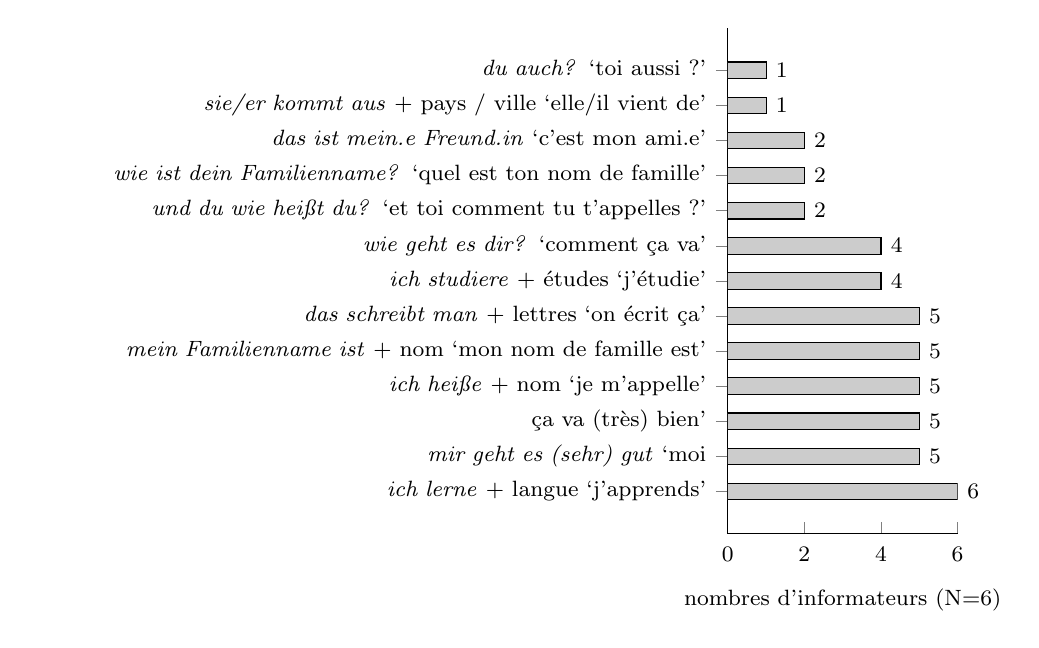
\begin{tikzpicture}
\begin{axis}[
    xbar,
    axis lines*=left,
    bar width = 6pt,
    xmin = 0,
    xmax = 6,
    width  = 4.5cm,
    height = 8cm,
    xlabel={nombres d'informateurs (N=6)},
    yticklabels = {\textit{ich lerne} + langue `j'apprends', \textit{mir geht es (sehr) gut} `moi, ça va (très) bien', \textit{ich heiße} + nom `je m'appelle', \textit{mein Familienname ist} + nom `mon nom de famille est', \textit{das schreibt man} + lettres `on écrit ça', \textit{ich studiere} + études `j'étudie', \textit{wie geht es dir?} `comment ça va', \textit{und du wie heißt du?} `et toi comment tu t'appelles ?', \textit{wie ist dein Familienname?} `quel est ton nom de famille', \textit{das ist mein.e Freund.in} `c'est mon ami.e', \textit{sie/er kommt aus} + pays / ville `elle/il vient de', \textit{du auch?} `toi aussi ?', \textit{er/sie lernt Deutsch} `il / elle apprend l'allemand'},
    ytick = data,
    typeset ticklabels with strut,
    yticklabel style={text width=8.5cm,align=right},
    tick label style={font=\footnotesize},
    nodes near coords,
    nodes near coords style={font=\footnotesize},
    nodes near coords align={horizontal},
    font=\footnotesize
      ]
      \addplot [draw=black, fill=black!20] coordinates {
        (6,0) 
        (5,1) 
        (5,2) 
        (5,3) 
        (5,4) 
        (5,5) 
        (4,6)
        (4,7)
        (2,8)
        (2,9)
        (2,10)
        (1,11)
        (1,12)
      };
\end{axis}
\end{tikzpicture}
\caption{Reprise de constructions présentes dans l'input\label{fig:felce:3a}}
\end{subfigure}\medskip\\
\begin{subfigure}{\textwidth}
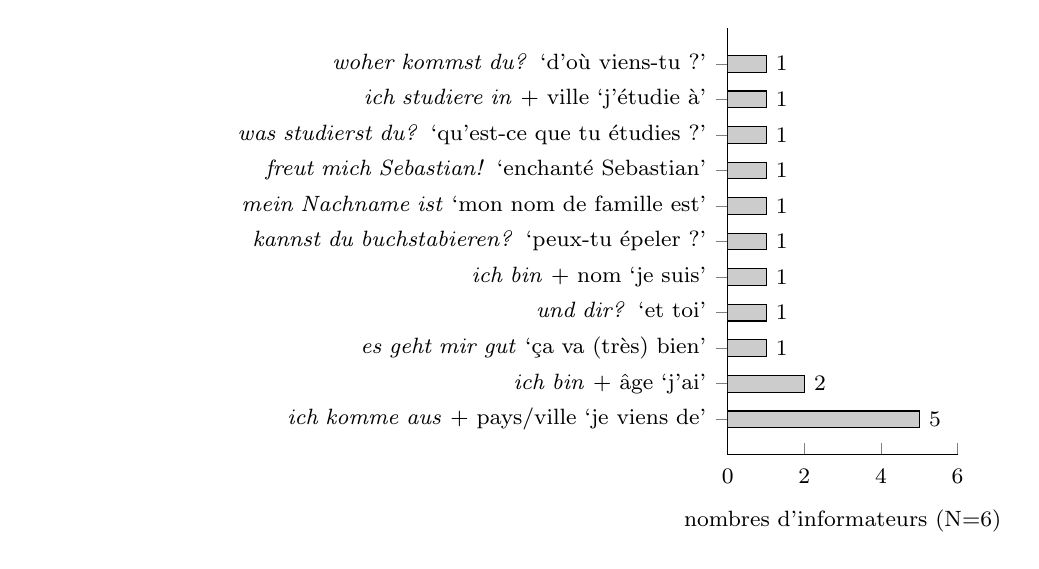
\begin{tikzpicture}
\begin{axis}[
    xbar,
    axis lines*=left,
    bar width = 6pt,
    xmin = 0,
    xmax = 6,
    width  = 4.5cm,
    height = 7cm,
    xlabel={nombres d'informateurs (N=6)},
    yticklabels = {\textit{ich komme aus} + pays/ville `je viens de', \textit{ich bin} + âge `j'ai', \textit{es geht mir gut} `ça va (très) bien', \textit{und dir?} `et toi', \textit{ich bin} + nom `je suis', \textit{kannst du buchstabieren?} `peux-tu épeler ?', \textit{mein Nachname ist} `mon nom de famille est', \textit{freut mich Sebastian!} `enchanté Sebastian', \textit{was studierst du?} `qu'est-ce que tu étudies ?', \textit{ich studiere in} + ville `j'étudie à', \textit{woher kommst du?} `d'où viens-tu ?'},
    ytick = data,
    typeset ticklabels with strut,
    yticklabel style={text width=8.5cm,align=right},
    tick label style={font=\footnotesize},
    nodes near coords,
    nodes near coords style={font=\footnotesize},
    nodes near coords align={horizontal},
    font=\footnotesize
      ]
      \addplot [draw=black, fill=black!20] coordinates {
        (5,0) 
        (2,1) 
        (1,2) 
        (1,3) 
        (1,4) 
        (1,5) 
        (1,6)
        (1,7)
        (1,8)
        (1,9)
        (1,10)
      };
\end{axis}
\end{tikzpicture}
\caption{Autres constructions mobilisées\label{fig:felce:3b}}
\end{subfigure}
\caption{Constructions observables dans la toute première tâche de production (tâche 1)\label{fig:felce:3}}
\end{figure}

On constate en effet que les expressions présentes dans le modèle de l’interlocutrice germanophone sont majoritairement reprises par les apprenants (\figref{fig:felce:3a}); d’autres constructions, en revanche, sont introduites pour exprimer la provenance (manipulée de manière privilégiée dans les activités effectuées en amont en classe), apporter d’autres informations (études, nom de famille, âge) ou gérer la tâche de manière plus personnelle (\figref{fig:felce:3b}). 

Si  certains apprenants se contentent de reproduire des phrases calquées sur le modèle de l’interlocutrice, d’autres sélectionnent en effet des constructions différentes de celles de l’input pour exprimer une même fonction comme en \REF{ex:felce:4}. INF21\_06 se place quant à lui dans une dynamique plus interactive en simulant un dialogue à partir de l’input fourni, ce qui explique l’intégration dans sa production de questions et de répliques qui viennent s’articuler ou réagir de manière créative à celles de l’interlocutrice fictive \REF{ex:felce:5}.

\ea%4
    \label{ex:felce:4}
    \ea \textit{ich bin} au lieu de \textit{ich heiße} … `je suis vs je m’appelle'
    \ex \textit{mein Nachname ist …} au lieu de \textit{mein Familienname ist …} `mon nom de famille'
     \z
\ex%5
    \label{ex:felce:5}
    \ea INPUT = \textit{das ist mein Freund, Sebastian. → freut mich, Sebastian!} `c’est mon ami … → enchanté…'
    \ex INPUT = \textit{er lernt Deutsch, du auch? → ja, *ich auch lerne Deutsch}  `il apprend l’allemand, toi aussi? → oui, moi aussi, j’apprends l’allemand'
    \z
\z


Il n’est pas non plus surprenant d’observer que les segments se caractérisent par une correction formelle, morphologique ou syntaxique. La morphologie verbale de la première personne \textit{ich} `je' ainsi que le placement verbal dans les questions et les assertions sont correctement réalisés, même dans le cas de certaines structurations spécifiques~qui demeurent à ce stade (+ 4h), non analysées (\textit{mir geht es gut} `moi, ça va bien', \textit{das schreibt man} `on écrit ça'). La fixité des reprises, associée à la correction formelle, laissent penser que les apprenants font usage d’exemplaires mémorisés (\citealt[88]{Myles2012}), utiles à une gestion immédiate et pragmatique de la tâche. La créativité s’exprime exclusivement dans le choix des informations ajoutées (âge, langues, ville d’origine par exemple) ou du format (dialogué ou monologal) que les apprenants ont voulu donner à leur production et ne vient pas affecter la forme ou le contenu lexical des constructions reprises.

\subsection{Une variété de constructions pour parler de soi}\label{sec:felce:6.2}

La deuxième tâche de production orale (\tabref{tab:felce:4}, tâche 2), administrée après 8 heures de cours, constitue à la fois une reprise et un prolongement de la tâche précédente. La modalité et la consigne sont similaires, mais une durée plus longue et une diversification des informations est attendue : il s’agit de réaliser à nouveau un portrait audio de soi en mobilisant les moyens langagiers ayant fait l’objet des interactions en cours (âge, origine, études, loisirs, langues connues ou apprises, souhaits, entre autres). Les exemples \REF{ex:felce:fromtab:7}, extraits du syllabus, montrent qu’un usage de structures spécifiques
(XVfinS ou SVfin-OVinf) est également visé.

\ea \label{ex:felce:fromtab:7}
  \ea Cadrer un propos\\
  \gll {\textit{wie geht’s \textbf{heute}?}}      {→}  {\textit{heute geht’s mir\slash heute bin ich} + adj}\\
  {`comment ça va \textbf{aujourd’hui}'}    {}        {`aujourd’hui ça va / je suis'}\\

  \ex Indiquer d’où on vient et où on habite maintenant\\
  \textit{ich komme aus} + pays/ville \textit{aber jetzt wohne ich in} + pays/ville\\\relax
  `je viens de … mais \textbf{maintenant} j’habite à '

  \ex Dire les langues que l’on parle ou apprend\\
  \textit{ich spreche / ich kann / ich lerne} + langue `je parle / je sais parler, j’apprends'\\
  \textit{jetzt lerne ich} \textbf{+} langue `maintenant, j’apprends'

  \ex Indiquer un souhait\\
  \textit{ich \textbf{möchte} / ich \textbf{will}} \textit{…. Japanisch} \textbf{\textit{lernen}} `je \textbf{voudrais} \textbf{/} \textbf{je} \textbf{veux} \textbf{apprendre} le japonais'
  \z
\z
 

La consigne donnée mentionne les attentes en termes de contenu et de durée et explique la plus grande variété des constructions employées que l’on peut observer (\figref{fig:felce:4}).

\begin{figure}
  \begin{subfigure}{\textwidth}
  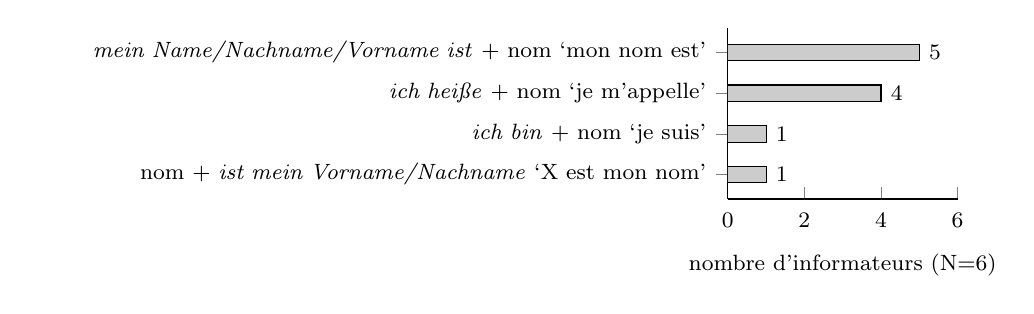
\begin{tikzpicture}
  \begin{axis}[
      xbar,
      axis lines*=left,
      bar width = 6pt,
      xmin = 0,
      xmax = 6,
      width = 4.5cm,
      height = 3.75cm,
      xlabel={nombre d'informateurs (N=6)},
      yticklabels = {{nom + \textit{ist mein Vorname/Nachname} `X est mon nom'},
                     {\textit{ich bin} + nom `je suis'},
                     {\textit{ich heiße} + nom `je m'appelle'},
                     {\textit{mein Name/Nachname/Vorname ist} + nom `mon nom est'}
                     },
      ytick = data,
      typeset ticklabels with strut,
      yticklabel style={text width=8.5cm,align=right},
      tick label style={font=\footnotesize},
      nodes near coords,
      nodes near coords style={font=\footnotesize},
      nodes near coords align={horizontal},
      font=\footnotesize,
      enlarge y limits=0.2
        ]
        \addplot [draw=black, fill=black!20] coordinates {
          (1,0) 
          (1,1)
          (4,2)
          (5,3)
        };
  \end{axis}
  \end{tikzpicture}
  \caption{Se présenter}
  \end{subfigure}\medskip\\
  % Removed as per author's request
 % % % % \begin{subfigure}{\textwidth}
% % % % \begin{tikzpicture}
% % % %  \begin{axis}[
% % % %      xbar,
% % % %      axis lines*=left,
% % % %      bar width = 6pt,
% % % %      xmin = 0,
% % % %      xmax = 6,
% % % %      width = 4.5cm,
% % % %      height = 3.5cm,
% % % %      xlabel={nombres d'occurrences},
% % % %      yticklabels = {{\textit{ich bin}+date de naissance `je suis'},
 % % % %                    {\textit{er/sie ist}+âge `il/elle a'},
% % % %                     {\textit{ich bin} +âge `j'ai'}},
% % % %      ytick = data,
% % % %      typeset ticklabels with strut,
% % % %      yticklabel style={text width=8.5cm,align=right},
% % % %      tick label style={font=\footnotesize},
% % % %      nodes near coords,
% % % %      nodes near coords style={font=\footnotesize},
% % % %      nodes near coords align={horizontal},
% % % %      font=\footnotesize,
% % % %      enlarge y limits=0.2
% % % %        ]
% % % %        \addplot [draw=black, fill=black!20] coordinates {
% % % %          (1,0) 
% % % %          (1,1)
% % % %          (6,2)
% % % %        };
% % % %  \end{axis}
% % % %  \end{tikzpicture}
% % % %  \caption{indiquer son âge}
% % % %  \end{subfigure}\medskip\\
  % Removed as per author's request
% % % %   \begin{subfigure}{\textwidth}
% % % %   \begin{tikzpicture}
% % % %   \begin{axis}[
% % % %       xbar,
% % % %       axis lines*=left,
% % % %       bar width = 6pt,
% % % %       xmin = 0,
% % % %       xmax = 6,
% % % %       width = 4.5cm,
% % % %       height = 2.75cm,
% % % %       enlarge y limits=0.5,
% % % %       xlabel={nombre de locuteurs (N=6)},
% % % %       yticklabels = {{\textit{ich buchstabiere} `j'épelle'},
% % % %                      {\textit{das schreibt man} `on écrit ça'},
% % % %                      },
% % % %       ytick = data,
% % % %       typeset ticklabels with strut,
% % % %       yticklabel style={text width=8.5cm,align=right},
% % % %       tick label style={font=\footnotesize},
% % % %       nodes near coords,
% % % %       nodes near coords style={font=\footnotesize},
% % % %       nodes near coords align={horizontal},
% % % %       font=\footnotesize
% % % %         ]
% % % %         \addplot [draw=black, fill=black!20] coordinates {
% % % %           (1,0) 
% % % %           (3,1)
% % % %         };
% % % %   \end{axis}
% % % %   \end{tikzpicture}
% % % %   \caption{épeler}
% % % %   \end{subfigure}\medskip\\

  \begin{subfigure}{\textwidth}
  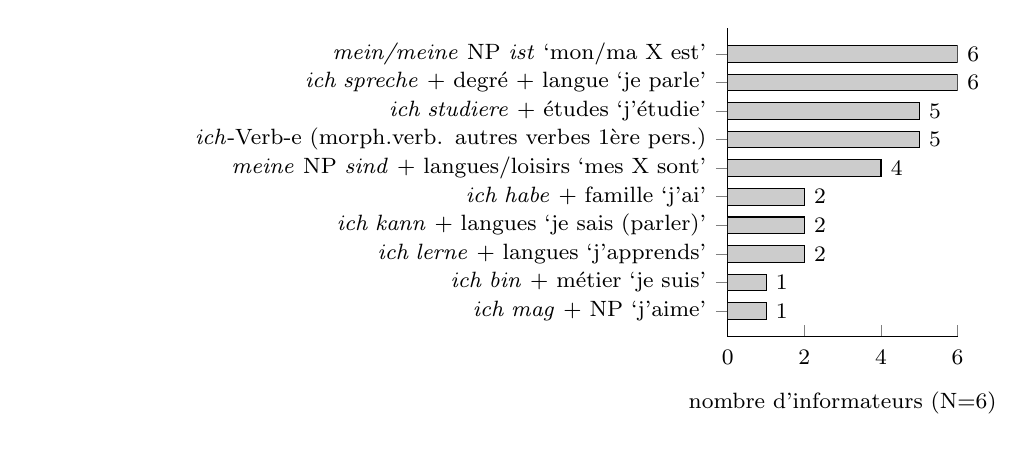
\begin{tikzpicture}
  \begin{axis}[
      xbar,
      axis lines*=left,
      bar width = 6pt,
      xmin = 0,
      xmax = 6,
      width = 4.5cm,
      height = 5.5cm,
      xlabel={nombre d'informateurs (N=6)},
      yticklabels = {{\textit{ich mag} + NP `j'aime'},
                     {\textit{ich bin} + métier `je suis'},
                     {\textit{ich lerne} + langues `j'apprends'},
                     {\textit{ich kann} + langues `je sais (parler)'},
                     {\textit{ich habe} + famille `j'ai'},
                     {\textit{meine} NP \textit{sind} + langues/loisirs `mes X sont'},
                     {\textit{ich}-Verb-e (morph.verb. autres verbes 1ère pers.)},
                     {\textit{ich studiere} + études `j'étudie'},
                     {\textit{ich spreche} + degré + langue `je parle'},
                     {\textit{mein/meine} NP \textit{ist} `mon/ma X est'}
                   },
      ytick = data,
      typeset ticklabels with strut,
      yticklabel style={text width=8.5cm,align=right},
      tick label style={font=\footnotesize},
      nodes near coords,
      nodes near coords style={font=\footnotesize},
      nodes near coords align={horizontal},
      font=\footnotesize
        ]
        \addplot [draw=black, fill=black!20] coordinates {
          (1,0) 
          (1,1)
          (2,2) 
          (2,3)
          (2,4)
          (4,5) 
          (5,6)
          (5,7) 
          (6,8)
          (6,9)
        };
  \end{axis}
  \end{tikzpicture}
  \caption{Donner des informations personnelles}
  \end{subfigure}\medskip\\
  
  \begin{subfigure}{\textwidth}
  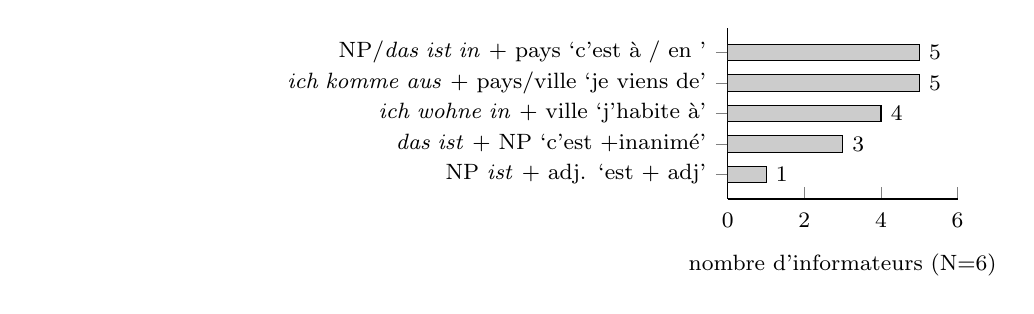
\begin{tikzpicture}
  \begin{axis}[
      xbar,
      axis lines*=left,
      bar width = 6pt,
      xmin = 0,
      xmax = 6,
      width = 4.5cm,
      height = 3.75cm,
      xlabel={nombre d'informateurs (N=6)},
      yticklabels = {{NP \textit{ist} + adj. `est + adj'},
                     {\textit{das ist} + NP `c'est +inanimé'},
                     {\textit{ich wohne in} + ville `j'habite à'},
                     {\textit{ich komme aus} + pays/ville `je viens de'},
                     {NP/\textit{das ist  in} + pays `c'est à / en '}},
      ytick = data,
      typeset ticklabels with strut,
      yticklabel style={text width=8.5cm,align=right},
      tick label style={font=\footnotesize},
      nodes near coords,
      nodes near coords style={font=\footnotesize},
      nodes near coords align={horizontal},
      font=\footnotesize,
      enlarge y limits=0.2
        ]
        \addplot [draw=black, fill=black!20] coordinates {
          (1,0) 
          (3,1)
          (4,2) 
          (5,3)
          (5,4)
        };
  \end{axis}
  \end{tikzpicture}
  \caption{Localiser}
  \end{subfigure}\medskip\\
  \begin{subfigure}{\textwidth}
  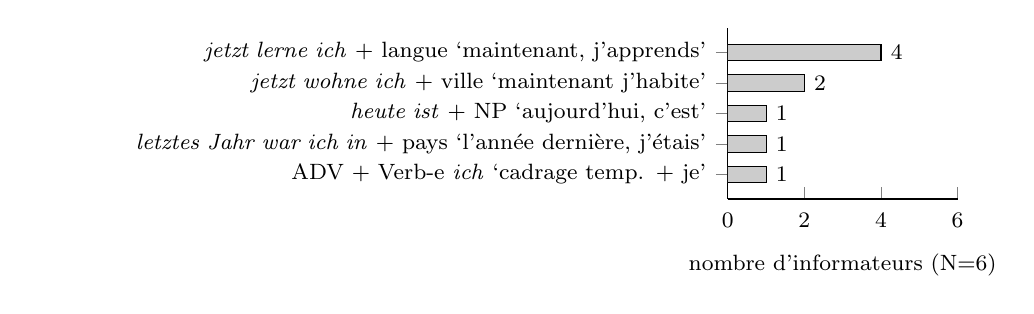
\begin{tikzpicture}
  \begin{axis}[
      xbar,
      axis lines*=left,
      bar width = 6pt,
      xmin = 0,
      xmax = 6,
      width = 4.5cm,
      height = 3.75cm,
      xlabel={nombre d'informateurs (N=6)},
      yticklabels = {{ADV + Verb-e \textit{ich} `cadrage temp. + je'},
                     {\textit{letztes Jahr war ich in} + pays `l'année dernière, j'étais'},
                     {\textit{heute ist} + NP `aujourd'hui, c'est'},
                     {\textit{jetzt wohne ich} + ville `maintenant j'habite'},
                     {\textit{jetzt lerne ich} + langue `maintenant, j'apprends'}},
      ytick = data,
      typeset ticklabels with strut,
      yticklabel style={text width=8.5cm,align=right},
      tick label style={font=\footnotesize},
      nodes near coords,
      nodes near coords style={font=\footnotesize},
      nodes near coords align={horizontal},
      font=\footnotesize,
      enlarge y limits = 0.2
        ]
        \addplot [draw=black, fill=black!20] coordinates {
          (1,0) 
          (1,1)
          (1,2) 
          (2,3)
          (4,4)
        };
  \end{axis}
  \end{tikzpicture}
  \caption{Cadrer dans le temps}
  % Removed as per author's request
% % % %   \end{subfigure}\medskip\\  
% % % %   \begin{subfigure}{\textwidth}
% % % %   \begin{tikzpicture}
% % % %   \begin{axis}[
% % % %       xbar,
% % % %       axis lines*=left,
% % % %       bar width = 6pt,
% % % %       xmin = 0,
% % % %       xmax = 6,
% % % %       width = 4.5cm,
% % % %       height = 2.75cm,
% % % %       xlabel={nombres d'occurrences},
% % % %       yticklabels = {{\textit{ich möchte}+NP* `je voudrais (une chose)'}, {\textit{ich möchte}+VP `je voudrais (faire)'}},
% % % %       ytick = data,
% % % %       typeset ticklabels with strut,
% % % %       yticklabel style={text width=8.5cm,align=right},
% % % %       enlarge y limits=0.5,
% % % %       tick label style={font=\footnotesize},
% % % %       nodes near coords,
% % % %       nodes near coords style={font=\footnotesize},
% % % %       nodes near coords align={horizontal},
% % % %       font=\footnotesize
% % % %         ]
% % % %         \addplot [draw=black, fill=black!20] coordinates {
% % % %           (1,0) 
% % % %           (2,1)
% % % %         };
% % % %   \end{axis}
% % % %   \end{tikzpicture}
% % % %  \caption{exprimer un souhait}
   \end{subfigure}
\caption{Variété des constructions mobilisées (tâche 2)\label{fig:felce:4}}
\end{figure}

 % Removed as per author's request
% % % % \begin{figure}\ContinuedFloat
% % % %   \begin{subfigure}{\textwidth}
% % % %   \begin{tikzpicture}
% % % %   \begin{axis}[
% % % %       xbar,
% % % %       axis lines*=left,
% % % %       axis lines*=left,
% % % %       axis lines*=left,
% % % %       bar width = 6pt,
 % % % %      xmin = 0,
% % % %       xmax = 6,
% % % %       width = 4.5cm,
% % % %       height = 3.75cm,
% % % %       xlabel={nombre d'informateurs (N=6)},
% % % %       yticklabels = {{NP \textit{ist} + adj. `est +adj'},
% % % %                      {\textit{das ist} +NP `c'est +inanimé'},
% % % %                      {\textit{ich wohne in} +ville `j'habite à'},
% % % %                      {\textit{ich komme aus}+pays/ville `je viens de'},
% % % %                      {NP/\textit{das ist  in}+ pays `c'est à / en '}},
% % % %       ytick = data,
% % % %       typeset ticklabels with strut,
% % % %       yticklabel style={text width=8.5cm,align=right},
% % % %       tick label style={font=\footnotesize},
% % % %       nodes near coords,
% % % %       nodes near coords style={font=\footnotesize},
% % % %       nodes near coords align={horizontal},
% % % %       font=\footnotesize,
% % % %       enlarge y limits=0.2
% % % %         ]
% % % %         \addplot [draw=black, fill=black!20] coordinates {
% % % %           (1,0) 
% % % %           (3,1)
% % % %           (4,2) 
% % % %           (5,3)
% % % %           (5,4)
% % % %         };
% % % %   \end{axis}
% % % %   \end{tikzpicture}
% % % %   \caption{localiser}
% % % %   \end{subfigure}\medskip\\
% % % %   \begin{subfigure}{\textwidth}
% % % %   \begin{tikzpicture}
% % % %   \begin{axis}[
% % % %       xbar,
% % % %       axis lines*=left,
% % % %       bar width = 6pt,
% % % %       xmax = 6,
% % % %       width = 4.5cm,
% % % %       height = 3.75cm,
% % % %       xlabel={nombre de locuteurs (N=6)},
% % % %       yticklabels = {{ADV+Verb-e \textit{ich} `cadrage temp. + je'},
% % % %                      {\textit{letztes Jahr war ich in} +pays `l'année dernière, j'étais'},
% % % %                      {\textit{heute ist}+NP `aujourd'hui, c'est'},
% % % %                      {\textit{jetzt wohne ich}+ville `maintenant j'habite'},
% % % %                      {\textit{jetzt lerne ich}+langue `maintenant, j'apprends'}},
 % % % %      ytick = data,
 % % % %      typeset ticklabels with strut,
% % % %       yticklabel style={text width=8.5cm,align=right},
% % % %       tick label style={font=\footnotesize},
% % % %       nodes near coords,
% % % %       nodes near coords style={font=\footnotesize},
% % % %       nodes near coords align={horizontal},
% % % %       font=\footnotesize,
% % % %       enlarge y limits = 0.2
% % % %         ]
 % % % %        \addplot [draw=black, fill=black!20] coordinates {
 % % % %          (1,0) 
 % % % %          (1,1)
% % % %           (1,2) 
% % % %           (2,3)
% % % %           (4,4)
% % % %         };
% % % %   \end{axis}
% % % %   \end{tikzpicture}
% % % %   \caption{cadrer dans le temps}
  % Removed as per author's request
% % % %   \end{subfigure}\medskip\\  
% % % %   \begin{subfigure}{\textwidth}
% % % %   \begin{tikzpicture}
% % % %   \begin{axis}[
% % % %       xbar,
% % % %       axis lines*=left,
% % % %       bar width = 6pt,
% % % %       xmin = 0,
% % % %       xmax = 6,
% % % %       width = 4.5cm,
% % % %       height = 2.75cm,
% % % %       xlabel={nombres d'occurrences},
% % % %       yticklabels = {{\textit{ich möchte}+NP* `je voudrais (une chose)'}, {\textit{ich möchte}+VP `je voudrais (faire)'}},
% % % %       ytick = data,
% % % %       typeset ticklabels with strut,
% % % %       yticklabel style={text width=8.5cm,align=right},
% % % %       enlarge y limits=0.5,
% % % %       tick label style={font=\footnotesize},
% % % %       nodes near coords,
% % % %       nodes near coords style={font=\footnotesize},
% % % %       nodes near coords align={horizontal},
% % % %       font=\footnotesize
% % % %         ]
% % % %         \addplot [draw=black, fill=black!20] coordinates {
% % % %           (1,0) 
% % % %           (2,1)
% % % %         };
% % % %   \end{axis}
% % % %   \end{tikzpicture}
% % % %   \caption{exprimer un souhait}
% % % %   \end{subfigure}
% % % % \caption{Variété des constructions mobilisées (tâche 2) -- suite}
% % % % \end{figure}


On peut noter cette fois que plusieurs formes sont utilisées pour exprimer une même action langagière \REF{ex:felce:6}. Quand il s’agit, par exemple, de se présenter ou d’indiquer les langues parlées, les informateurs n’ont plus recours à une unique expression mais mobilisent des formulations distinctes selon les apprenants. 

\ea%6
    \label{ex:felce:6}
    \ea  \textit{ich heiße} + nom / prénom / OU prénom + \textit{ist mein Vorname} \\
    \relax  `je m’appelle OU est mon prénom'
    \ex  \textit{meine Muttersprache ist} + langue / \textit{ich spreche} + langue / \textit{ich kann auch} + langue \\
    \relax  `ma langue maternelle est / je parle / je sais aussi parler'
    \z
 \z

Le fait qu’il s’agisse ici d’une tâche formative pour laquelle les apprenants ont pu consulter des ressources explique certainement la variété observée. Néanmoins, des choix ont été faits et articulés par les apprenants pour réaliser la production attendue ; en ce sens, cette manipulation constitue un événement d’usage pour les formes et expressions mobilisées.

On peut par ailleurs constater le recours fréquent à une construction de type \textit{mein/meine} NP + \textit{ist/sind} `mon/ma/mes + est/sont' qui indique que cette construction constitue un patron dans lequel des éléments personnels variés peuvent être introduits (nom / adresse / téléphone / courriel / langues / loisirs). 

Entre la tâche 1, où l’emploi de \textit{mein} n’était associé qu’à la mention du nom (\textit{mein Name / mein Familienname} `mon nom / mon nom de famille') et la tâche 2, on est passé d’une instance spécifique à un schéma plus ouvert et disponible pour l’expression d’une variété d’informations. Les réalisations orales montrent dans la majorité des cas une différentiation dans le marquage du féminin ou du pluriel sur le déterminant possessif, respectivement \textit{meine} vs \textit{mein}. L’alternance entre \textit{meine} et \textit{mein,} et entre \textit{ist} et \textit{sind} `est /sont' pour la forme verbale associée, met en évidence un certain degré de productivité du schéma \textit{mein}- + NP + \textit{ist / sind} dont les différentes réalisations relèvent d’une variation de type.

Enfin, on constate que certains apprenants font aussi le choix de réinvestir des constructions présentant un cadrage temporel. Ces constructions (\textit{jetzt lerne ich Deustch} `maintenant j’apprends l’allemand' / \textit{jetzt wohne ich in +} ville `maintenant j’habite à') ont été volontairement introduites lors des échanges en classe. Le but de cette introduction précoce est de solliciter la répétition d’associations Verbe-Sujet dans des configurations avec la première personne (\textit{ich} `je') et il est intéressant de voir \REF{ex:felce:7} que des apprenants ont cherché à reproduire de telles options de linéarisation dans des formulations différentes de celles abordées en classe.

\ea%7
    \label{ex:felce:7}
    \ea \textit{am Wochenende gehe ich} \textit{+} activité `le week-end, je vais'
    \ex \textit{in meiner Freizeit höre ich Musik} `dans mon temps libre, j’écoute de la musique'
    \ex \textit{heute ist mein Geburtstag} `aujourd’hui, c’est mon anniversaire'
    \ex \textit{letztes Jahr war ich} + lieu `l’année dernière, j’étais'
\z
\z

\subsection{Disponibilité et adaptation des constructions}\label{sec:felce:6.3}
\begin{sloppypar}
Si l’on confronte ensuite les résultats de la tâche formative de production orale qui précède à la première tâche de production écrite évaluée (tâche 3a), on constate une réduction des moyens langagiers (\figref{fig:felce:5}).
\end{sloppypar}

\vfill
\begin{figure}[H]
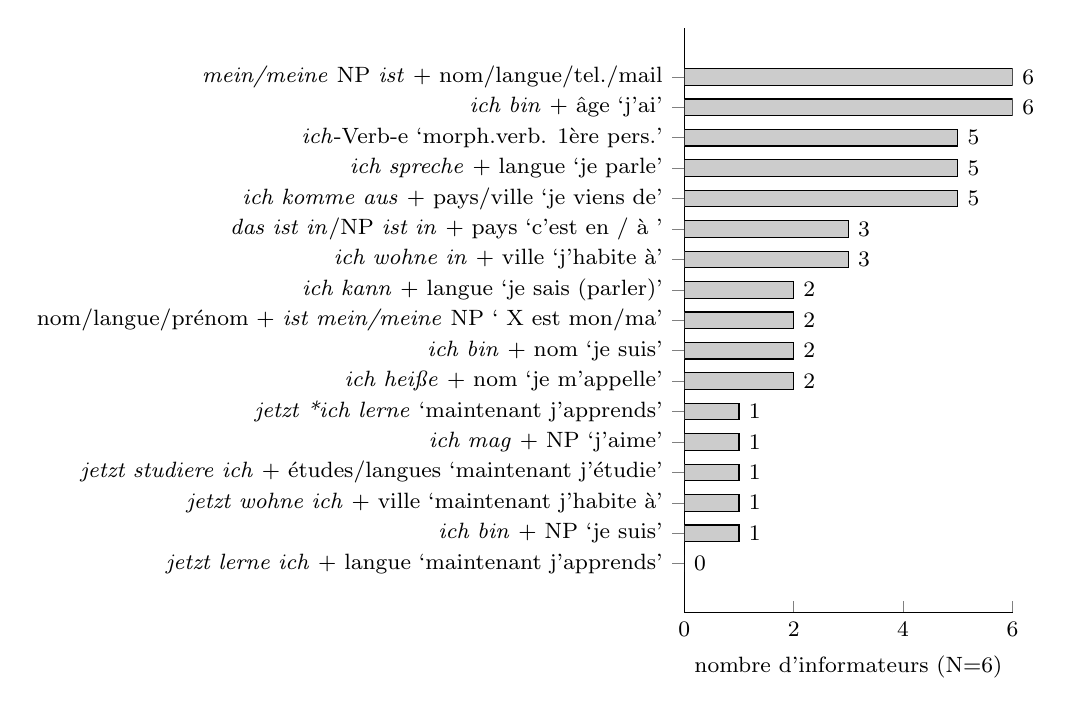
\begin{tikzpicture}
\begin{axis}[
    xbar,
    axis lines*=left,
    bar width = 6pt,
    xmin = 0,
    xmax = 6,
    width = 5.75cm,
    height = 9cm,
    xlabel={nombre d'informateurs (N=6)},
    yticklabels = {{\textit{jetzt lerne ich} + langue `maintenant j'apprends'},
                   {\textit{ich bin} + NP `je suis'},
                   {\textit{jetzt wohne ich} + ville `maintenant j'habite à'},
                   {\textit{jetzt studiere ich} + études/langues `maintenant j'étudie'},
                   {\textit{ich mag} + NP `j'aime'},
                   {\textit{jetzt *ich lerne} `maintenant j'apprends'},
                   {\textit{ich heiße} + nom `je m'appelle'},
                   {\textit{ich bin} + nom `je suis'},
                   {nom/langue/prénom + \textit{ist mein/meine} NP  ` X est mon/ma'},
                   {\textit{ich kann} + langue `je sais (parler)'},
                   {\textit{ich wohne in} + ville `j'habite à'},
                   {\textit{das ist in}/NP \textit{ist in} + pays `c'est en / à '},
                   {\textit{ich komme aus} + pays/ville `je viens de'},
                   {\textit{ich spreche} + langue `je parle'},
                   {\textit{ich}-Verb-e `morph.verb. 1ère pers.'},
                   {\textit{ich bin} + âge `j'ai'},
                   {\textit{mein/meine} NP \textit{ist} + nom/langue/tel./mail}
                   },
    ytick = data,
    tick label style={font=\footnotesize},
    nodes near coords,
    nodes near coords style={font=\footnotesize},
    nodes near coords align={horizontal},
    font=\footnotesize
      ]
      \addplot [draw=black, fill=black!20] coordinates {
        (0,0) 
        (1,1)
        (1,2)
        (1,3)
        (1,4) 
        (1,5)
        (2,6)
        (2,7)
        (2,8) 
        (2,9)
        (3,10)
        (3,11)
        (5,12)
        (5,13) 
        (5,14)
        (6,15)
        (6,16)
      };
\end{axis}
\end{tikzpicture}
\caption{Constructions disponibles et mobilisées en situation de production contrôlée (tâche 3a)\label{fig:felce:5}}
\end{figure}
\vfill
\pagebreak

Cette réduction peut être attribuée à la tâche elle-même (brièveté du format d’une annonce, éléments informatifs mis bout à bout, manque de consignes sur le contenu ou le format attendue) ; les conditions de production (en temps limité et sans consultation de ressources) sont également des facteurs qui ont pu favoriser le recours à des expressions plus disponibles ou plus productives que d’autres. Ainsi, les constructions à partir des formes du verbe être \textit{ich bin / das ist} `je suis / c’est' sont par exemple mobilisées en lien avec plusieurs informations (âge, caractéristiques, occupation, localisation) ; \textit{ich bin} `je suis' est par ailleurs utilisé par deux informateurs pour se présenter, alors que cette expression n’avait été employée qu’au tout début des présentations de soi et avait très vite cédé la place dans les usages à d’autres formulations (\textit{ich heiße / mein Name ist} `je m’appelle / mon nom est').\largerpage

On observe à nouveau de nombreux emplois du patron \textit{mein/meine} + NP \textit{ist} `mon/ma + NP est', disponible pour indiquer plusieurs informations personnelles (le nom, le numéro de téléphone, l’email, la langue maternelle). Ces constructions ont été répétées maintes fois dans les séances de cours et leur fréquence d’usage est accrue par le fait qu’elles couvrent justement plusieurs notions ; par ailleurs leur brièveté, leur simplicité formelle ou leur proximité phonologique avec l’anglais (\textit{my/mein}) peuvent aussi expliquer la facilité d’emploi.

\begin{sloppypar}
En ce qui concerne les aspects morphosyntaxiques, on note une préférence marquée pour des réalisations de type SVfin qui débutent par le sujet \textit{ich} `je'. \citet{Winkler2017} fait remarquer qu’il est difficile d’éviter de mettre en avant \textit{ich} quand, en début d’apprentissage, les apprenants sont invités à parler d’eux-mêmes. Les formes verbales en nombre limitées sont correctement réalisées, ce qui semble confirmer le fait que les apprenants mobilisent ici des tournures apprises et mémorisées telles quelles, sans qu’elles ne soient décomposées ni analysées.
\end{sloppypar}

Une deuxième partie de l’évaluation (tâche 3b) consiste en une autre production écrite qui vise cette fois la caractérisation simple d’autres personnes (\textit{er}/\textit{sie} `il/elle') à partir d’informations fournies sous forme de mots-clés (identité, provenance, études, langues, âge).

\begin{figure}
\begin{subfigure}{\textwidth}
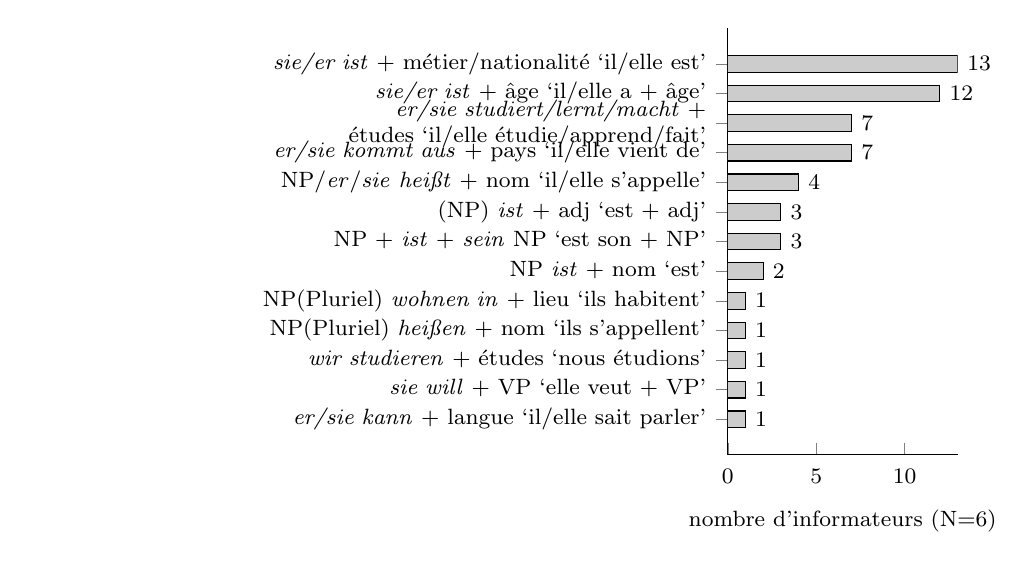
\begin{tikzpicture}
\begin{axis}[
    xbar,
    axis lines*=left,
    bar width = 6pt,
    xmin = 0,
    xmax = 13,
    width = 4.5cm,
    height = 7cm,
    xlabel={nombre d'informateurs (N=6)},
    yticklabels = {{\textit{er/sie kann} + langue `il/elle sait parler'},
                   {\textit{sie will}  + VP `elle veut + VP'},
                   {\textit{wir studieren} + études `nous étudions'},
                   {NP(Pluriel) \textit{heißen} + nom `ils s'appellent'},
                   {NP(Pluriel) \textit{wohnen in} + lieu `ils habitent'},
                   {NP \textit{ist} + nom `est'},
                   {NP + \textit{ist} + \textit{sein} NP `est son + NP'},
                   {(NP) \textit{ist} + adj  `est + adj'},
                   {NP/\textit{er}/\textit{sie} \textit{heißt} + nom `il/elle s'appelle'},
                   {\textit{er/sie kommt aus} + pays `il/elle vient de'},
                   {\textit{er/sie studiert/lernt/macht} + études `il/elle étudie/apprend/fait'},
                   {\textit{sie/er  ist} + âge `il/elle a + âge'},
                   {\textit{sie/er ist} + métier/nationalité `il/elle est'}
    },
    ytick = data,
    typeset ticklabels with strut,
    yticklabel style={text width=8.5cm,align=right},
    tick label style={font=\footnotesize},
    nodes near coords,
    nodes near coords style={font=\footnotesize},
    nodes near coords align={horizontal},
    font=\footnotesize
      ]
      \addplot [draw=black, fill=black!20] coordinates {
        (1,0) 
        (1,1)
        (1,2) 
        (1,3)
        (1,4) 
        (2,5)
        (3,6) 
        (3,7)
        (4,8) 
        (7,9)
        (7,10) 
        (12,11)
        (13,12)
      };
\end{axis}
\end{tikzpicture}
\caption{Stabilité\label{fig:felce:6a}}
\end{subfigure}\medskip\\
\begin{subfigure}{\textwidth}\raggedright
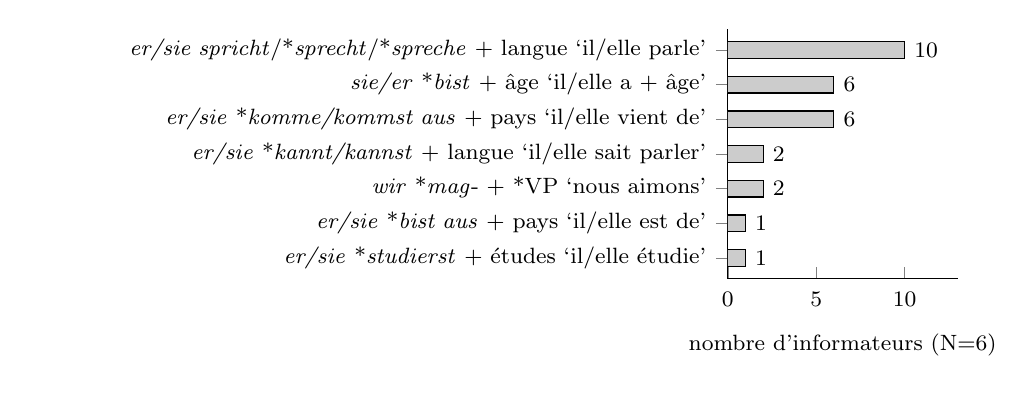
\begin{tikzpicture}
\begin{axis}[
    xbar,
    axis lines*=left,
    bar width = 6pt,
    xmin = 0,
    xmax = 13,
    width = 4.5cm,
    height = 4.75cm,
    xlabel={nombre d'informateurs (N=6)},
    yticklabels = {{\textit{er/sie} *\textit{studierst} + études `il/elle étudie'},
                   {\textit{er/sie} *\textit{bist aus} + pays `il/elle est de'},
                   {\textit{wir} *\textit{mag}- + *VP `nous aimons'},
                   {\textit{er/sie} *\textit{kannt/kannst} + langue `il/elle sait  parler'},
                   {\textit{er/sie} *\textit{komme/kommst aus} + pays   `il/elle vient de'},
                   {\textit{sie/er} *\textit{bist} + âge `il/elle a + âge'},
                   {\textit{er/sie spricht}/*\textit{sprecht}/*\textit{spreche} + langue `il/elle parle'},
                   },
    ytick = data,
    typeset ticklabels with strut,
    yticklabel style={text width=8.5cm,align=right},
    tick label style={font=\footnotesize},
    nodes near coords,
    nodes near coords style={font=\footnotesize},
    nodes near coords align={horizontal},
    font=\footnotesize
      ]
      \addplot [draw=black, fill=black!20] coordinates {
        (1,0) 
        (1,1)
        (2,2) 
        (2,3)
        (6,4)
        (6,5)
        (10,6)
      };
\end{axis}
\end{tikzpicture}
\caption{Alternance de formes\label{fig:felce:6b}}
\end{subfigure}
\caption{Stabilité vs alternance des formes verbales au sein des constructions (tâche 3b)\label{fig:felce:6}}
\end{figure}

Ce qui semble intéressant ici, c’est l’observation des variations dans la morphologie verbale à la 3\textsuperscript{ème} personne du singulier. En effet, si des formes verbales semblent afficher une certaine stabilité (\figref{fig:felce:6a}) qui peut être attribuée à la fréquence d'usage (\textit{ist}) ou à une relative simplicité formelle, d'autres se caractérisent en revanche par une grande variabilité, observable à travers  une alternance de formes distinctes de la 1ère personne, mais le plus souvent inadéquates pour le marquage de la 3ème pers. (\figref{fig:felce:6b}).
 
Un seul informateur sur les six (INF21\_06) réalise en effet correctement le marquage verbal aux trois personnes du singulier pour une variété de verbes \REF{ex:felce:new-ex-1}.

\ea\label{ex:felce:new-ex-1}
     \ea \textit{ich bin in + lieu / ich lebe in + lieu / ich studiere} + langue `je suis / je vis / j’étudie'
     \ex \textit{er/sie ist} + nom/âge/nationalité /métier `il/elle est'
     \ex \textit{er/sie kommt aus} + pays `el/elle vient de'
     \ex \textit{er/sie studiert} + études   `il/elle étudie'
     \ex \textit{er/sie lernt} + langue `il/elle apprend'
     \ex \textit{er/sie macht} + cursus `il/elle fait'
     \ex \textit{wo wohnst du? / was studierst du?} `où habites-tu ? / qu’étudies-tu ?'
     \z
\z

Ces réalisations affichent un fort degré de contrôle de la correction verbale et semblent montrer un traitement plus analytique des énoncés produits chez cet apprenant. Chez tous les autres, on observe que des formes correspondant aux deux premières personne (\textit{ich} Verb\textit{-e} `je' ; \textit{du} Verb\textit{-st} `tu') se substituent dans certaines constructions à celles de la 3\textsuperscript{ème} personne \REF{ex:felce:9} alors qu’un marquage de la 3\textsuperscript{ème} personne est par ailleurs parfois bien réalisé. 

\ea%9
    \label{ex:felce:9}
     \ea NP \textit{heißt} + nom / sie ist + âge / \textit{sie studiert} + études / \textit{sie *kommst aus} + pays `s’appelle / elle a / elle étudie / elle vient de'
     \ex\relax NP *\textit{komme aus} + pays / \textit{sie *studierst} + études `vient de / elle étudie'
     \ex\relax NP \textit{kommt aus} + pays / \textit{sie *spreche} + langue  `vient de / elle parle'
     \z
\z


L’usage privilégié des formes des deux premières personnes n’est pas surprenant dans la mesure où elles ont été manipulées en priorité dans les premières heures de cours. Ce qui apparaît là, c’est que certaines constructions initialement apprises à la première personne (\textit{ich komme aus} + pays `je viens de' ; \textit{ich spreche} + langue `je parle') ne sont pas affectées par le changement de personne, elles restent fixes alors que pour d’autres constructions, des tentatives de modification et de recherche d’une forme adéquate sont observables individuellement à travers l’alternance flexionnelle.

\subsection{Apparition de réalisations syntaxiques spécifiques}\label{sec:felce:6.4}\largerpage[2]

La dernière tâche écrite évaluative (tâche 4) vient clore le premier semestre d’apprentissage de la langue. En amont de cette tâche, des constructions relatives à ce que l’on souhaite boire ou manger ont été introduites et ont permis l’usage d’expressions cadratives \REF{ex:felce:10a} ou cohésives \REF{ex:felce:10b}, ainsi que de la structure du groupe verbal (OVinf) \REF{ex:felce:11}.

\ea%10
    \label{ex:felce:10}
    \ea \textit{zum Frühstück esse ich} + NP `au petit-déjeuner, je prends' \label{ex:felce:10a}
    \ex \textit{dazu nehme ich/trinke ich/möchte ich} + NP `avec ça je prends/je bois/je voudrais'\label{ex:felce:10b}
    \z
\ex%11
    \label{ex:felce:11}
    \ea \textit{möchtest du + einen Kaffee trinken?} `est-ce que tu voudrais boire un café ?'
    \ex \textit{ich möchte + etwas bestellen} `je voudrais commander quelque chose'
    \z
\z

Un dernier ensemble d’activités menées en classe a également sollicité la manipulation de constructions utiles à la localisation spatiale \REF{ex:felce:12}.

\ea%12
    \label{ex:felce:12}
   \ea \textit{in der ersten Etage befindet sich} + NP `au premier étage se trouve'
   \ex \textit{ganz oben gibt es} + NP `tout en haut il y a'
   \ex \textit{im zweiten Stock ist / sind} + NP `au deuxième étage est / sont'
   \ex \textit{da kann man / kannst du / können Sie} + OVinf `là, on peut / tu peux / vous pouvez'
    \z
\z

Toutes ces constructions sont censées réactiver l’emploi d’associations Verbe-Sujet dans un nouveau contexte, en lien avec de nouvelles actions langagières et banaliser encore un peu plus l’emploi de constituants distincts du sujet à l’ouverture.

La consigne associée à cette tâche spécifie le cadre et les attentes : les apprenants font un séjour à Berlin et écrivent une carte postale ou un email dans lequel ils décrivent les personnes qu’ils rencontrent, l’hôtel dans lequel ils sont logés, le buffet du petit déjeuner. La tâche de production est précédée d’une tâche de compréhension portant sur une brochure de l’hôtel, si bien que des éléments lexicaux sont disponibles dans cet input et peuvent être réinvestis par les apprenants. Les segments strictement identiques à ceux présents dans le texte ont été exclus de l’analyse de manière à ne considérer que les réalisations correspondant aux choix opérés par les apprenants à partir de ce matériau verbal.

\begin{table}
\small%
\caption{Émergence de réalisations syntaxiques spécifiques (tâche 4)\label{tab:felce:7}}
\begin{tabular}{ll}
    \lsptoprule
	options de  & \\
	linéarisation & constructions utilisées\\\midrule
	\multicolumn{2}{l}{poser le contexte}\\\midrule
	SVfinO &  \textit{ das/}NP\textit{/er/sie + ist/sind} + adj /nom/age/métier `\textit{S ist/sind} + adj'\\
	&    NP/\textit{wir/er/sie} + Vfin `nous/il/elle'                           \\
	&   \textit{ich bin (jetzt) in} + lieu `je suis maintenant à'                \\
	XVfinS & \textit{jetzt bin ich in} + ville/lieu `maintenant je suis à '\\
	& \textit{mir geht es gut} `moi ça va bien'                    \\
	& \textit{in} + lieu \textit{macht sie} + NP `à + lieu elle fait'           \\\addlinespace
	\multicolumn{2}{l}{décrire le lieu}\\\midrule
	XVfinS & \textit{in} + lieu \textit{gibt es/befindet sich/ist}  + NP `dans + lieu il y a/se trouve/est'\\
	& \textit{in}+lieu  \textit{finde ich} + NP `dans + lieu je trouve'\\
	SVfin  & NP + \textit{befindet sich /ist in} + lieu `se trouve/est dans'\\
	XSVfin & lieu + \textit{ich habe} + NP ` lieu + j'ai'\\
	& lieu + \textit{ich kann} + VinfO `lieu + je peux'\\\addlinespace
	\multicolumn{2}{l}{cadrer le propos}\\\midrule
	XSVfinO & \textit{heute} + lieu \textit{ich} + Vfin `aujourd'hui + lieu + je'\\
	& \textit{morgens wir haben} + NP `le matin, nous avons' \\
	XVfinSO & \textit{zum Frühstück haben wir} + NP `au petit-déjeuner nous avons'\\\addlinespace
	\multicolumn{2}{l}{lier à ce qui précède}\\\midrule
	XVfinSO & \textit{wo kann ich/wo finden wir} `où je peux/nous trouvons'\\
	&  \textit{da kann man} + VP `là on peut'\\
	&  \textit{dann habe ich/dazu trinke ich} + NP `après j'ai/avec ça je bois'\\
	& \textit{dazu kann ich} + VinfO `en plus je peux'\\\addlinespace
	\multicolumn{2}{l}{séparation des éléments verbaux (SEP)}\\\midrule
	SVfin-VinfO & \textit{ich kann} + VinfO `je peux'\\
	& \textit{er kann} + VinfO `il peut' \\
	SVfin-OVinf & \textit{man muss} + OVinf `on doit'\\
	\lspbottomrule
	\end{tabular}
\end{table}

Le relevé des expressions utilisées (\tabref{tab:felce:7}) montre que l’on retrouve à nouveau dans les productions des apprenants des constructions apprises lors des premières heures de cours, répétées et désormais maitrisées. Par ailleurs, et contrairement aux tâches initiales qui ont été analysées, on observe cette fois de nombreuses expressions qui correspondent à des choix de linéarisation spécifiques de l’allemand, à savoir : une attaque de l’énoncé par un adverbial faisant office de cadre temporel ou spatial pour le contenu propositionnel \REF{ex:felce:14a} ou par des éléments anaphoriques assurant à la fois la cohésion avec ce qui précède et l’ancrage situationnel de l’énoncé \REF{ex:felce:14b}.

\ea%14
    \label{ex:felce:14}
    \ea \label{ex:felce:14a} \textit{\textbf{jetzt} bin ich in} + lieu `maintenant, je suis à'
    \ex \label{ex:felce:14b} \textit{… der *Garden und \textbf{da} kann man ein Bier trinken} `…le jardin et là on peut boire une bière'
    \z
\z

Pour décrire le lieu (l’hôtel), les apprenants alternent entre une structuration canonique \REF{ex:felce:15a} et une linéarisation partant de points de repère pour la localisation d’autres éléments (\ref{ex:felce:15b}--\ref{ex:felce:15d}).

\ea%15
    \label{ex:felce:15}
     \ea \label{ex:felce:15a} \textit{ein Frühstücksraum ist in} + lieu `une salle pour le petit-déjeuner est'
     \ex\label{ex:felce:15b} \textit{im Erdgeschoss gibt es} + NP `au rez-de-chaussée il y a'
     \ex\label{ex:felce:15c}\textit{in der ersten Etage, *ich habe} + NP `au premier étage, j’ai'
     \ex\label{ex:felce:15d}\textit{im zweiten Stock befindet sich} + NP `au deuxième étage se trouve'
     \z
\z

Ces expressions relatives à la localisation ont certes été présentées et manipulées en classe sous cette forme, mais les apprenants les ont mémorisées avec plus ou moins de précision, comme en témoigne l’usage de certaines formes verbales. On observe en effet une cohabitation entre des formes correctes et stabilisées \textit{lieu + befindet sich / gibt es} + NP et des assemblages plus incertains, comme en \REF{ex:felce:16}. 

\ea%16
    \label{ex:felce:16}
    \textit{in mein Hotel, *finde sind} + NP `dans mon hôtel se trouve'
\z


\begin{figure}
\pgfplotstableread{data/felce-fig-8.csv}{\felcetableeight}
\begin{tikzpicture}
  \begin{axis}[
      ybar,
      width=\textwidth,
      axis lines*=left,
      xticklabels from table={\felcetableeight}{Data},
      xtick=data,
      height=7cm,
      ymin=0,
      bar width=1ex,
      cycle list name=langsci6]
      \addplot table [x expr=\coordindex, x=Data,y=INF21_01] {\felcetableeight};
      \addlegendentry{INF21\_01}
      \addplot table [x expr=\coordindex, x=Data,y=INF21_02] {\felcetableeight};
      \addlegendentry{INF21\_02}
      \addplot table [x expr=\coordindex, x=Data,y=INF21_03] {\felcetableeight};
      \addlegendentry{INF21\_03}
      \addplot table [x expr=\coordindex, x=Data,y=INF21_04] {\felcetableeight};
      \addlegendentry{INF21\_04}
      \addplot table [x expr=\coordindex, x=Data,y=INF21_05] {\felcetableeight};
      \addlegendentry{INF21\_05}
      \addplot table [x expr=\coordindex, x=Data,y=INF21_06] {\felcetableeight};
      \addlegendentry{INF21\_06}
  \end{axis}
\end{tikzpicture}
\caption{Principales réalisations syntaxiques présentes dans les segments transcrits (tâche 4). \label{fig:felce:7}}
\end{figure}

Si l’on observe enfin la répartition des options syntaxiques choisies (\figref{fig:felce:7}), on constate que les linéarisations SVfin restent prédominantes sur le total des segments pris en compte pour chaque informateur, mais il apparait aussi qu’à côté d’options syntaxiques non conformes (X(PP /Adv)-SVfin), des choix de linéarisation pertinents semblent se mettre en place \REF{ex:felce:17}. Ces choix se font certes de manière inégale selon les individus, mais avec une certaine variété dans les formes mobilisées ; on note par ailleurs aussi que la linéarisation choisie contribue à établir une contiguïté et par là une continuité de sens au fil du texte caractéristique de la LC (\citealt[1642]{ZifonunEtAl1997}).\largerpage

\ea%17
    \label{ex:felce:17}
    \ea[*]{\textit{In der Mehrbettzimmer ist} + prénom →\textit{mit wir ist} + prénom\\\relax
    `dans le dortoir il y a'                                   `avec nous il y a'}

   \ex[]{\textit{Sie ist *studentin.} → \textit{In der Universität macht sie einen Bachelor.}\\\relax
    `Elle est étudiante.'                      `À la fac, elle fait une licence'}
    \z
\z

Malgré la difficulté d’une telle tâche de production pour le niveau A1, les performances semblent montrer des évolutions vers non pas plus de correction, mais plus d’adéquation à des options de linéarisation pertinentes dans le contexte du texte ou du discours.

\section{Discussion}\label{sec:felce:7}

La discussion portera principalement sur les données issues des tâches d’évaluation effectuées en classe et en temps limité (45 min.) dans la mesure où les apprenants doivent recourir pour ces productions aux seuls moyens langagiers disponibles dans leur interlangue.

Les résultats obtenus permettent de mettre en évidence des évolutions pour lesquelles la variation de la morphologie verbale semble être un signe. À l’issue des premières heures de cours, on constate que des constructions sont réemployées sous une forme qui semble se limiter à la reproduction des premières constructions apprises. Relativement rapidement cependant (+ 8 heures) des variations peuvent être observées : au moment où des expressions pour parler des autres s’ajoutent à celles pour parler de soi, la perception qu’ont les apprenants de la nécessité de faire usage de nouvelles formes verbales vient modifier des constructions initialement figées et spécifiques. Cette variation de la morphologie verbale au sein des constructions peut être interprétée comme le signe d’un échange d’information grammaticale entre les constituants qui marquerait le début d’une transformation d’exemplaires au départ fortement lexicalisés en instances plus analysées et plus grammaticalisées. 

L’évolution des constructions semble cependant soumise fortement aux différences individuelles évoquées en introduction. L’un sera plus ou moins sensible à la répétition d’une forme, ou à la variation de type pour une même instance. On peut se demander ce qui, au-delà de ces différences, fait en sorte qu’une construction puisse être apprise et devienne disponible pour la production langagière. En ce qui concerne \textit{ich bin} `je suis' ou \textit{mein/meine ist} `mon/ma est', la brièveté, la simplicité ou la proximité phonologique avec l’anglais, ainsi que le fait qu’il s’agisse de constructions plurifonctionnelles constituent très certainement des facteurs facilitant la mémorisation et le rappel et expliquant la fréquence d’usage observée.

Il est remarquable que des formes de la deuxième personne \textit{bist / kommst} / \textit{studierst} (pour les verbes `être, venir, étudier'), connues pour avoir été manipulées dans les questions, se substituent parfois à celles de la 3\textsuperscript{ème} personne. La proximité sonore des terminaisons de la 2\textsuperscript{ème} et 3\textsuperscript{ème} personne (respectivement \textit{-st /-t}) les rend moins saillantes et peut favoriser le manque de distinction pour les exemples relevés. 

Au-delà de ce constat, il est aussi possible de faire l’hypothèse que certains apprenants, conscients de la nécessaire adaptation de la construction au changement de personne, n’utilisent pour cela plus les formes mémorisées de la 1\textsuperscript{ère} personne~et aient alors recours aux autres formes les plus disponibles dans leur répertoire langagier pour combler le déficit ou le rappel moins automatisé de la forme verbale adéquate. La variabilité dans les formes pourrait alors s'apparenter à des tentatives d'adaptation opérées par les apprenants sur les formes à partir de ce dont ils disposent et la morphologie de la 2\textsuperscript{ème} personne du singulier ferait ainsi figure de forme « par défaut » (\citealt{vanderVelde2004}) tant que la flexion correcte de la 3\textsuperscript{ème} personne n’est pas acquise.

\begin{sloppypar}
Un deuxième aspect concerne le développement schématique des constructions. Les premières productions semblent s’appuyer sur des instances spécifiques, mémorisées telles quelles pour l’expression de fonctions particulières et nécessairement modestes au tout début~de l’apprentissage ; avec l’apparition d’autres besoins, le nombre d’instances à mémoriser augmente et justifie le recours à des patrons afin de réduire le coût mémoriel engagé. À partir de l’analyse des segments produits dans les différentes tâches, il semble possible de distinguer des degrés dans la schématicité des constructions identifiées et de reconnaitre une évolution de certaines de ces constructions vers des patrons plus ouverts à de nouvelles combinaisons (\tabref{tab:felce:9}). Les constructions repérées semblent ainsi pouvoir relever de trois niveaux : 
\end{sloppypar}\largerpage

\begin{itemize}
\item \textit{un niveau 0} correspondant à un degré de spécificité élevé et à l’usage de constructions sous leur forme lexicale, sans modification ;
\item \textit{un niveau 1} caractérisant des constructions fixes mais pouvant être complétées par l’ajout d’éléments sémantiquement homogènes ;
\item \textit{un niveau 2} regroupant, d’une part, des expressions dont certains éléments constitutifs peuvent être modifiés pour s’adapter à la situation de communication et, d’autre part, des constructions pouvant être mobilisées pour des fonctions sémantiques ou pragmatiques différentes ; 
\item \textit{et un niveau 3} relatif aux constructions attestant d’une relative abstraction, identifiable à travers un patron qui se répète dans des usages distincts.
\end{itemize}

\begin{sidewaystable}
\caption{Exemples de schématisation progressive dans les productions analysées\label{tab:felce:9}} 
\small
\begin{tabularx}{\textwidth}{QQQl}
    \lsptoprule
    {Niveau 0} & {Niveau 1} & {Niveau 2} & {Niveau 3}\\\midrule
    \textit{jetzt wohne ich in Frankreich}
    
    `maintenant, j’habite en France' & \textit{jetzt wohne/lebe ich in + pays}
    
    `maintenant, j’habite\slash je vis' & \rdelim\}{3}{*}[\parbox{.25\textwidth}{\raggedright \textit{jetzt\slash heute\slash zum Frühstück\slash morgens} + Vfin (\textit{ich\slash er\slash sie\slash wir}) + NP `maintenant\slash aujourd’hui\slash au petit-déjeuner\slash le matin + Vfin (je\slash il\slash elle\slash ils\slash elles\slash nous) + NP'}] & \rdelim\}{8}{*}[\parbox{1.75cm}{Adv + Vfin + S + NP (+ PP) (+ NP) (+ adj.)}]\\
    \textit{zum Frühstück trinke ich Kaffee}
    
    `au petit-déjeuner, je bois du café' & \textit{zum Frühstück\slash morgens + trinke ich\slash nehme ich} + NP
    
    `au petit-déjeuner / le matin, je bois / je prends + NP' &  & \\\addlinespace
    \textit{im Hostel gibt es eine Lounge}
    
    `à l’hotel, il y a un salon' & in + lieu \textit{gibt es\slash finden wir} + NP
    
    `il y a / nous trouvons + NP' & lieu + Vfin S + NP & \\\addlinespace
    \textit{da kann man ein Bier trinken}
    
    `là on peut boire une bière'
    
    \textit{in der Lounge kann man im Internet surfen }
    
    `dans le salon, on peut surfer sur Internet' & \textit{da\slash dann} + \textit{kann man\slash ich\slash können wir} + OVinf\slash VP
    
    `là/ensuite + on peut/je peux/ nous pouvons + VP' & \textit{da\slash dann} + Vfin (\textit{ich\slash wir\slash er\slash sie}) + OVinf/VP & \parbox{1.75cm}{Adv + Vfin + S (+ OVinf)} \\\addlinespace
    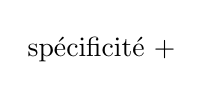
\begin{tikzpicture}[remember picture, baseline=(felce-node-table-specific.base)] 
    \node [inner xsep=0pt] (felce-node-table-specific) {spécificité +}; \end{tikzpicture} & & & 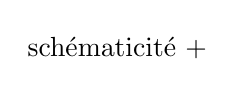
\begin{tikzpicture}[remember picture, baseline=(felce-node-table-schematic.base)] 
    \node [inner xsep=0pt] (felce-node-table-schematic) {schématicité\vphantom{p} +}; \end{tikzpicture}\\
    \lspbottomrule
\end{tabularx}
\begin{tikzpicture}[remember picture, overlay]
   \draw[{Triangle[]}-{Triangle[]}] (felce-node-table-specific.east) -- (felce-node-table-schematic.west);
\end{tikzpicture}
\end{sidewaystable}

\begin{sloppypar}
Enfin, même si certaines constructions idiosyncrasiques peuvent donner l’impression de n’être que des épiphénomènes, leur usage témoigne néanmoins d’évolutions intéressantes qui semblent s’inspirer de modèles plus stabilisés. Les formulations \REF{ex:felce:18} pourraient en effet être assimilées aux constructions de type (\textit{da kann man} `là on peut', \textit{in +} lieu \textit{finden wir} `à + lieu + nous trouvons') et être catégorisées par certains apprenants sous un même patron productif.
\end{sloppypar}

\ea%18
    \label{ex:felce:18}
     \ea \textit{im Garten, *wo kochen wir} + NP `un jardin, où nous cuisinons'
     \ex \textit{eine Lounge, *wo kann ich +} VP `un lobby, où je peux'
     \ex \textit{eine Rezeption, *wo finden wir} + NP `un accueil où nous trouvons'
     \z
\z

Les exemples illustrés en \REF{ex:felce:18} représentent ainsi, chez deux informateurs, des tentatives de formation de propositions relatives qui semblent s’appuyer sur les constructions ADV-Vfin-S (XVfinS) manipulées et qui pourraient être utilement mises à profit par l’enseignant pour l’apport de connaissances explicites relatives au positionnement final des formes verbales finies dans les subordonnées (O + (Vinf) + Vfin).

\section{Conclusion}\label{sec:felce:8}

L’étude menée part de pratiques enseignantes mises en œuvre avec des apprenants débutant l’allemand en contexte universitaire. L’approche privilégiée leur permet de manipuler différentes expressions langagières dans des usages communicatifs variés. Les activités d’enseignement et les tâches ont été considérées comme des événements d’usage, c’est-à-dire des occasions d’exposition à et de pratique de la langue qui participent de l’apprentissage et de l’évolution du système langagier des apprenants. À partir d’un corpus constitué à partir de cinq productions (2 tâches orales et 3 tâches écrites) de six apprenants inscrits dans un cours d’allemand grands débutants à l’université, les constructions utilisées dans les productions analysées ont été répertoriées et l’émergence de nouvelles combinaisons a été mise en évidence, en rapport avec les options de linéarisation des constituants de l’énoncé.

\begin{sloppypar}
Les données transcrites et segmentées ont été analysées en fonction des constructions pouvant être associées aux actions langagières visées au niveau A1, en fonction des formes verbales utilisées dans ces constructions et de la structuration syntaxique des énoncés produits (Annexe~\ref{felce:appendix:A}). Les résultats montrent que : 
\end{sloppypar}

\begin{itemize}\sloppy
\item les premières formes sont d’autant plus facilement mémorisées et réemployées qu’elles sont simples, brèves et plurifonctionnelles,

\item une évolution est observable entre des constructions réemployées sans modification lexicale en dépit du changement de personne et des constructions à l’intérieur desquelles les formes verbales s’avèrent plus mouvantes ; ces tâtonnements ont été interprétés comme le signe d’une transition d’instances figées vers des patrons plus ouverts,

\item la manipulation de constructions permettant d’assigner à l’ouverture de l’énoncé une fonction cadrative, situative (temporelle ou locale) ou de continuité informationnelle donne lieu à des combinaisons individuelles qui semblent s’inspirer de schémas pouvant être perçus comme similaires et qui sont susceptibles de préparer des acquisitions syntaxiques plus complexes.
\end{itemize}

Par ailleurs, le travail de recensement mené a aussi permis d’établir différents degrés de schématisation pouvant être utiles à des analyses ultérieures dans le cadre théorique convoqué (\tabref{tab:felce:9}).

Ce travail est en ce sens exploratoire qu’il part de ce qu’il est possible d’observer dans un corpus de productions d’apprenants pour proposer des catégories d’analyse qui ne sont pas élaborées a priori. Les analyses menées appréhendent des performances d’apprenants débutants à partir de la notion de constructions et de schématicité \citep{Legallois2021} et inscrivent l’enseignement de la langue débutée dans une perspective inspirée de l’usage (\citealt{TylerOrtega2018}). La mémorisation initiale d’associations forme-sens, initialement sous la forme d’éléments lexicaux semble confirmer certaines anticipations formulées. Des évolutions se dessinent dans la succession des tâches, elles mériteraient d’être étudiées de manière plus approfondie~ou d’être complétées par des protocoles expérimentaux, mais l’adoption d’une approche constructionniste du développement permet :

\begin{itemize}\sloppy
  \item de considérer que des apprenants débutants peuvent être confrontés très tôt à des formes spécifiques de la LC sans attendre d’être équipés de connaissances grammaticales minimales (\citealt{Ellis2020} : 4),
  \item de comprendre que l’appropriation met en jeu des mécanismes cognitifs généraux (analogie, catégorisation, schématisation) qui peuvent demeurer implicites, mais aussi trouver à s’articuler avec une information grammaticale plus explicite dans le cadre de la classe de langue,
  \item de voir dans les premières acquisitions un apprentissage d’expressions lexicales qui évoluent vers des schématisations dans un processus de grammaticalisation graduelle, 
  \item d’offrir aux apprenants débutants des opportunités de pouvoir saisir des formes traditionnellement considérées comme complexes par d’autres biais que des règles formelles. 
\end{itemize}

\begin{sloppypar}\noindent
S'interroger sur la manière d’aborder différemment l’apprentissage d’une langue débutée en contexte guidé, c'est défendre l’idée qu’il peut s’agir d’une question d’usage(s) à plus d’un titre. L’usage concerne en premier lieu la perspective choisie et conditionne une conception de l’appropriation langagière qui resitue lexique et grammaire dans un continuum. À cette perspective s’articule une conception dynamique du système grammatical qui trouve sa source dans la linguistique cognitive et les grammaires de construction. La grammaire est ainsi vue comme un système évolutif constitué, à ses débuts, d’instances spécifiques liées à des usages particuliers, mais ouvert aux innovations que les différentes expériences d’usage vécues par les individus contribuent à construire et recomposer. L’usage s’applique également à l’intervention, c’est-à-dire aux occasions de rencontre et d’emploi de la LC que l’enseignant va chercher à solliciter chez l’apprenant à travers des interactions et des tâches significatives. Mais l’usage peut aussi renvoyer à des habitudes ou à des préconisations pour l’enseignement qui peuvent être remises en question et évoluer à travers un engagement dans des recherches de terrain ou par le biais de travaux directement utiles et accessibles aux enseignants.
\end{sloppypar}

\section*{Remerciements}
C’est dans le cours de Daniel Véronique à Paris 3, que je découvre en 2007 l’existence d’un domaine de recherche s’intéressant à la manière dont les individus s’approprient une langue seconde. Alors enseignante de langue, je n’ai encore jamais entendu parler d’acquisition, encore moins d’enseignabilité ; les apports de ce cours transformeront profondément ma vision de la langue et de son enseignement. Au-delà, les réflexions de Daniel marqueront aussi l’orientation de ma carrière et le positionnement qui est le mien, entre didactique et acquisition.

Je tiens à remercier les éditeurs de la série ainsi que les évaluateurs anonymes pour leur relecture détaillée des versions antérieures. Leurs commentaires et leurs conseils m'ont été d'une grande aide pour améliorer la forme et le contenu de ce chapitre.

\appendixsection{Guide des différents niveaux d’annotation des segments transcrits}\label{felce:appendix:A}

\begin{table}[H]
\caption{Constructions identifiées [constr.]}
\begin{tabularx}{\textwidth}{QQ}
\lsptoprule
action langagière visée (\textit{Sprachhandlung}) & annotations\\\midrule
dire comment ça va & mir geht’s + adj\\
se présenter & ich heiße + nom\\
présenter qn & das ist + nom ; er/sie heißt + nom\\
donner des informations personnelles ou sur autrui (origine, ville ou lieu de résidence, langues, âge, occupation, études, ce qu’on aime) & ich/er/sie bin/ist/sind + âge/métier/adj/in + lieu\\\addlinespace
& ich/er/sie komme/kommt aus + pays/ville ; ich/er/sie wohne/wohnt in + lieu ; ich/er/sie mag NP\\\addlinespace
décrire ce que l’on fait (activités diverses) & NP Verb NP\\\addlinespace
décrire / caractériser des lieux & das ist + adj ; NP haben NP* (il y a); NP ist + adj\\\addlinespace
préciser le temps et le lieu & in + lieu gibt es NP ; NP befindet sich in + lieu ; temps *wir haben + NP\\
\lspbottomrule
\end{tabularx}
\end{table}

\begin{table}
\caption{Organisation informationnelle  [org.]}
\begin{tabularx}{\textwidth}{QQ}
\lsptoprule
fonction & annotations\\\midrule
cadrage spatio-temporel & jetzt bin ich in + lieu; jetzt lerne ich + langue\\
cohésion (avec une information qui précède) & Cornflakes ↔ dazu trinke ich  + NP\\
\lspbottomrule
\end{tabularx}
\end{table}

\begin{table}
\caption{Structuration syntaxique (ordre des mots) [synt.]}
\begin{tabularx}{\textwidth}{Ql}
\lsptoprule
structure type & annotations\\\midrule
ordre canonique & SVO\\
inversion & XVfinSO\\
antéposition d’un constituant sans inversion & XSVfinO\\
souhait/possibilité + groupe infinitif & SVfin + OVinf\\
antéposition d’un constituant + verbe modal sans inversion + groupe infinitif & XSVfin + OVinf\\
séparation (SEP) : souhait/possibilité + infinitif + complément & SVfin + Vinf + O\\
\lspbottomrule
\end{tabularx}
\end{table}

\begin{table}
\caption{Correction morphosyntaxique [morph.]}
\begin{tabularx}{\textwidth}{QQ}
\lsptoprule
morphologie verbale & annotations\\\midrule
formes du verbe \textit{sein} ; \textit{haben} `être; avoir' (conformes ou non conformes) & bin / bist / ist /sind ; habe / *habe / hast / hat / *habt /haben / *haben / *bin / *bist/ *ist / *sind\\\addlinespace
formes des verbes \textit{können} `savoir faire/pouvoir' / \textit{möchten} `voudrais' & kann / *kann / *kannt / können / kannst /
möchte / *möchte / *möchtet / möchten\\\addlinespace
1ère pers. conforme ; non conforme & Verb-e ; *Verb-e\\
2ème pers. conforme ; non conforme  & Verb-st ; *Verb-st\\
3ème pers. sing conforme ; non conforme  & Verb-t ; *Verb-t  \\
pluriel conforme ; non conforme  & Verb-en ; *Verb-en\\
\lspbottomrule
\end{tabularx}
\end{table}

\printbibliography[heading=subbibliography,notkeyword=this]
\end{otherlanguage}
\end{document} 
